
		\chapter{Definition Mechanische Welle}

Eine Mechanische Welle\index{Welle!mechanische}\index{Mechanische Welle} tritt dann auf, wenn ein \emph{Wellenträger}\footnote{Es kann sich dabei um feste, flüssige oder gasförmige Materie handeln}\index{Wellenträger} eine \emph{Störung}\index{Störung} weiterleitet, ohne dass dabei die Teilchen des Wellenträgers wandern - sie bewegen sich nur am Ort. Dabei wird Energie\footnote{kinetische und potentielle Energie} transportiert. Die Geschwindigkeit, mit der sich die einzelnen Teilchen des Wellenträgers bewegen, wird als \emph{Schnelle} \(\vec{v}\)\index{Schnelle} bezeichnet.

Eine Welle breitet sich dabei mit einer bestimmten \emph{Ausbreitungsgeschwindigkeit} \(c\)\index{Ausbreitungsgeschwindigkeit} aus. Diese ist vom Wellenträger abhängig.\footnote{Es kann auch dazu kommen, dass die Ausbreitungsgeschwindigkeit von der Frequenz der Schwingung abhängt; das bezeichnet man als \emph{Dispersion}\index{Dispersion}.} Es kann dabei sein, dass sich nur eine einzelne Störung ausbreitet, es kann sich aber auch um einen periodischen Vorgang handeln.

\index{Longitudialwellen}\index{Transversalwellen}\index{Querwellen}\index{Längswellen}Man unterscheidet dabei zwischen Longitudinal- oder Längswellen und Transversal- bzw. Querwellen. Bei \emph{Longitudinal}wellen bewegen sich die Teilchen des Wellenträgers \emph{in} Ausbreitungsrichtung, bei \emph{Transversal}wellen bewegen sie sich senkrecht zur Ausbreitungsrichtung.



		\chapter{Feder-Massen-Modell}

Das Feder-Massen-Modell\index{Feder-Massen-Modell} dient dazu, sich die Ausbreitung einer Störung vorstellen zu können: In diesen Modell liegen Massenteilchen in einer Reihe und werden von Federn miteinander verbunden. Wird nun eines dieser Teilchen angeregt - bspw. nach oben gezogen -, so spricht man hier von einer Störung - schließlich wurde die geradlinige Anordnung der Teilchen gestört. Durch die Feder dieses ersten Massenteilchens zu seinem Nachbarn - durch die Störung wurde sie gespannt - wird dieser nun nach oben gezogen, wodurch er die nächste Feder spannt, die nun wiederum den nächsten Massenpunkt nach oben zieht. Durch die Trägheit der Massen der einzelnen Teilchen vergeht ein gewisser Zeitraum, bis ein Massenteilchen so weit ausgelenkt ist, wie sein Nachbar\footnote{daraus resultiert die Ausbreitungsgeschwindigkeit}. Auf diese Weise breitet sich die anfängliche Störung durch den kompletten Wellenträger aus - sieht man von Reibung u.ä. ab.




		\chapter{Harmonische Wellen}

Eine \emph{Fortschreitende Welle}\index{Fortschreitende Welle} ist das, was man sich für gewöhnlich unter dem Begriff ``Welle'' vorstellt. Dabei wird dem Wellenträger periodisch Energie zugeführt und die Massenteilchen bewegen sich mit gleichartigen, erzwungenen Schwingungen. Handelt es sich bei diesen Schwingungen der einzelnen Massenteilchen um harmonische Schwingungen, so wird die Welle als \emph{Harmonische Welle}\index{Harmonische Welle} bezeichnet.

Ein bestimmter Schwingungszustand\footnote{Das entspricht einem Bestimmten Winkel \(\varphi\) im Zeigerformalismus\index{Zeigerformalismus} (Kap. \ref{sss_zeigerdarstellung}).} breitet sich dabei mit der Geschwindigkeit \(c\) aus. Betrachtet man also zwei Teilchen, die genau \(c \cdot t_1\) auseinanderliegen, und phasengleich schwingen\footnote{also jederzeit mit dem selben Winkel \(\varphi\) darstellbar sind}, so muss es sich bei \(t_1\) um ein Vielfaches von der \emph{Schwingungsdauer} \(T\) handeln. \(T\) ist der kürzeste zeitliche Abstand zwischen zwei Teilchen, die phasengleich schwingen. Die kürzeste Distanz zwischen zwei Teilchen, die Phasengleich schwingen, wird als \emph{Wellenlänge} \(\lambda\) bezeichnet. Es gilt als Zusammenhang

\begin{equation}
 	c = \frac{\lambda}{T} = \lambda \cdot f
 	\label{eq_cLf}
\end{equation}


			\section{Wellengleichung}

\index{Wellengleichung!Mechanische Welle}Nun lässt sich einfach eine Wellengleichung herleiten, die dazu dient, die Auslenkung eines beliebigen Teilchens einer Welle zu einer beliebigen Zeit zu bestimmen. Dazu nimmt man an, dass die Welle sich linear ausbreitet und zwar in positive \(x\)-Richtung. Bei \(x =0\) wird die Welle periodisch angeregt, zum Zeitpunkt \(t = 0\) wird sie das erste mal in positive \(s\)-Richtung ausgelenkt.

Am Punkt \(x = 0\) schwingt das Teilchen also mit einer harmonischen Schwingung. Seine Amplitude ist \(\hat{s}\) und seine Drehfrequenz ist \(\omega\), dadurch beträgt sein Drehwinkel \(\varphi\) zum Zeitpunkt \(t\):  \(\varphi = \omega \cdot t\).  Die Gleichung zu seiner Schwingung lautet somit:
\begin{equation}
 	s(t) = \hat{s} \cdot sin(\omega \cdot t)
		\label{eq_s(t,x0)}
\end{equation}
Dieses Teilchen regt nun seine Nachbarn in positiver \(x\)-Richtung an und überträgt seine Bewegung darauf. Da sich diese Ausbreitung mit der Geschwindigkeit \(c\) vollzieht, hat jedes Teilchen, das vom ersten weiter als
\begin{equation}
 	x(t) = c \cdot t \Rightarrow t(x) = \frac{x}{c}
		\label{eq_x(t)}
\end{equation}
entfernt ist, keine Auslenkung - die erste Störung ist noch nicht bis zu ihm durchgedrungen.

Betrachtet man nun ein Teilchen, das nach Formel \ref{eq_x(t)} schon schwingen muss, so kann man auf dessen Auslenkung ganz einfach schließen, indem man berechnet, wie lange die Welle sich vom ersten Teilchen bis hierher ausgebreitet hat. Diese Dauer ergibt sich mit Formel \ref{eq_x(t)}. Aus der bereits verstrichenen Zeit \(t\) und dieser Zeit ergibt sich die Zeit, zu der das Teilchen an der Stelle \(x = 0\) den gesuchten Schwingungszustand hatte. Somit setzt man diese Zeit in Formel \ref{eq_s(t,x0)} ein, und erhält die gesuchte Auslenkung:
\begin{equation}
	s(x,t) = \hat{s} \cdot sin\left(\omega \cdot \left(t - \frac{x}{c}\right)\right) = \hat{s} \cdot sin\left(\frac{2 \cdot \pi}{T} \cdot \left(t - \frac{x}{\frac{\lambda}{T}}\right)\right) = \hat{s} \cdot sin\left(2 \cdot \pi \cdot \left(\frac{t}{T} - \frac{x}{\lambda}\right)\right)
		\label{eq_s(x,t)}
\end{equation}
Die Umformung erhält man mit \(\omega = \frac{2 \cdot \pi}{T}\) und \(c = \frac{\lambda}{T}\).

Diese Formel beschreibt nun für eine Schwingung die Auslenkung für beliebige Zeitpunkte und an beliebigen Orten. Sie kann auf drei verschiedene Arten verwendet werden:
\begin{enumerate}
 \item Auslenkung eines einzelnen Punktes zu einer Bestimmten Zeit:\\
	Dazu muss man in die Formel schlicht Abstand \(x\) vom ersten angeregten Teilchen und die Zeit \(t\) seit dem Beginn von dessen Anregung.

\item Ein Momentanbild der Schwingung erzeugen:\\
	Hierzu gibt man schlicht die Zeit seit Beginn der Anregung des ersten Teilchens in die Formel ein und wird eine \(s(x)\)-Gleichung erhalten. Dabei muss man aber beachten, dass diese Gleichung zum Schaubild einer Sinus-Welle gehört, die in beide Richtungen ins Unendliche geht. Die Welle ist zu einem Bestimmten Zeitpunkt aber noch nicht so weit fortgeschritten. Ab einem bestimmten Punkt (mit Formel \ref{eq_x(t)} zu berechnen), sind die Teilchen noch nicht ausgelenkt.

\item Die Schwingung eines speziellen Teilchens in der Zeit erzeugen:\\
	Hierbei geht man entsprechend vor - man setzt den \(x\)-Wert des Teilchens ein und beachtet dabei, dass vor \(t = 0\) keine Schwingung stattgefunden haben kann, sondern erst ab der durch Formel \ref{eq_x(t)} zu bestimmenden Zeit.
\end{enumerate}




\subsubsection{Phasenverschiebung}

\index{Phasenverschiebung}Bei den Berechnungen für eine Wellengleichung sind wir stets davon ausgegangen, dass das Teilchen bei \(x = 0\) zum Zeitpunkt \(t = 0\) angeregt wird und vorher noch nicht ausgelenkt war. Ist dies nicht der Fall, so muss man dies als \emph{Phasenverschiebung}\footnote{Im Prinzip die Phasendifferenz zum idealen Zustand.} berücksichtigen. Sie drückt sich in einem Winkel \(\varphi_0\) aus, der als konstanter Wert stets zum Drehwinkel \(\omega \cdot t\) addiert wird:
\begin{equation}
 	\varphi(t) = \omega \cdot t + \varphi_0
\end{equation}
Hat ein Massenteilchen an \(x = 0\) bei \(t = 0\) bereits die Auslenkung \(s_1\), so beträgt die Phasenverschiebung 
\begin{equation}
 	\varphi_0 = sin^{-1}\left (\frac{s_1}{\hat{s}} \right )
\end{equation}








			\section{Zeigerdarstellung}
			\label{sss_zeigerdarstellung}

\index{Zeigerformalismus!Definition}Dadurch, dass die einzelnen Massenteilchen der Harmonischen Welle harmonische Schwingungen ausführen, lassen sie sich auch leicht mit dem Zeiger-Formalismus darstellen. Jedem einzelnen Teilchen wird ein gedachter, im Kreis rotierender Zeiger zugeordnet, dessen Länge der Maximalen Auslenkung des Teilchens entspricht. Die Rotationsfrequenz des Zeigers entspricht der Frequenz des schwingenden Teilchens. Der Anteil des Zeigers, parallel zur Schnelle, entspricht der Auslenkung des einzelnen Teilchens.






		\chapter{Reflexion}
		
		
				\section{Festes Ende}


\index{Reflexion}\index{Festes Ende}Bei einer Reflexion an einem festen Ende drehen sich sowohl Schnelle \(v\), als auch Ausbreitungsrichtung \(c\) um. Dabei zieht das letzte - befestigte - Wellenträgerteilchen seine letzten Vorgänger zurück in die Ausgangslage, nachdem sie von der Schnelle bewegt wurden. Dieses \textit{Zurückgezogen-Werdens} des Wellenträgers wird damit zur neuen Schnelle.
				
				\section{Loses Ende}

\index{Loses Ende}Bei Reflexion am losen Ende dagegen, behält die Schnelle \(v\) ihre Richtung bei, während nur die Ausbreitungsgeschwindigkeit \(c\) ihre Richtung umkehrt. Hierbei können sich die letzten Wellenträger frei bewegen. Sie werden von der Schnelle bewegt, und ziehen ihre Vorgänger dann mit in die selbe Richtung; dieses \textit{Mitgezogen-Werden} wird hierbei zur neuen Schnelle.


				\section{Konstruktionshilfe}
				
Zur Konstruktion einer durch Reflektion resultierenden Welle gibt es kleine Tricks. Dazu stellt man sich die Welle einfach weiter hinter dem reflektierenden Ende vor. Der \textit{'überschüssige'} Wellenteil wird dann
\begin{description}
 \item[Festes Ende] am festen Punkt punktgespiegelt.
 \item[Loses Ende] an der Achse, auf der sich das lose Ende bewegt, gespiegelt.
 \end{description}
Diese Spiegelungen addiert man dann schlicht zu der hinlaufenden Welle und hat als Resultierende Welle die Reflexion.

Um diese reflektierten Wellen mathematisch auszudrücken kann man analog zu Formel \ref{eq_s(x,t)} auf S. \pageref{eq_s(x,t)} die folgenden Formeln verwenden. Für Reflektion am \emph{festen Ende} gilt:
\begin{equation}
 	s_r(x,t) = - \hat{s} \cdot sin\left(2 \cdot \pi \cdot \left(\frac{t}{T} - \frac{(2 \cdot L - x)}{\lambda}\right)\right)
\end{equation}
Und für Reflektion am \emph{losen Ende} gilt:
\begin{equation}
 	s_r(x,t) = \hat{s} \cdot sin\left(2 \cdot \pi \cdot \left(\frac{t}{T} - \frac{(2 \cdot L - x)}{\lambda}\right)\right)
\end{equation}
Bei der Reflektion gibt es jedoch zu bedenken, dass die reflektierte Welle nach der Zeit \(t_1\) erst eine bestimmte Strecke \(x_1\) zurückgelegt hat, so dass sie erst \emph{ab} dem folgenden Punkt schwingt:
\begin{equation}
 	x_1 = 2 \cdot L - c \cdot t_!
\end{equation}




				\section{Im Zeigerformalismus}

\index{Zeigerformalismus!Reflexion}Im Zeigerformalismus sieht eine Reflexion beim festen und losen Ende unterschiedlich aus. Beim \emph{festen Ende} erfolgt ein so genannter \textit{Phasensprung}. Das bedeutet, dass an dem Teilchen, an dem reflektiert wird, der Zeiger der herlaufenden Welle genau in die Gegenrichtung zeigt, wie der Zeiger der reflektierten Welle. Das ist logisch, da die Summe der beiden Vektoren an dieser Stelle einen Nullvektor ergeben muss.

Bei Reflektion am \emph{losen Ende} dagegen, tritt der Phasensprung nicht auf. Hier kann das letzte Teilchen sich frei bewegen. Die Zeiger für hinlaufende und reflektierte Welle sind an dieser Stelle identisch - deshalb ergibt sich hier auch eine doppelt so hohe Amplitude.






		\chapter{Überlagerung}
		
\index{Ueberlagerung von Wellen@Überlagerung von Wellen}\index{Interferenz}Treffen zwei Störungen oder Wellen auf einem Wellenträger aufeinander, so durchdringen sie sich ungestört. Dabei addieren sich jedoch die Elongationen und Schnellen der beiden Wellen - es sieht aus, als hätte man eine neue Welle. Diesen Vorgang bezeichnet man als \emph{Interferenz}


		\section{Eindimensionaler Wellenträger}

\subsubsection{Gleichlaufende Wellen}
\label{par_Gleichlaufende Wellen}

Laufen zwei Wellen in die gleiche Richtung und haben darüber hinaus noch die selbe Wellenlänge \(\lambda\), so unterscheiden sie sich voneinander durch den \emph{Gangunterschied}\index{Gangunterschied} \(\delta\) bzw. die Phasendifferenz \(\Delta \varphi\)\index{Phasendifferenz}. Der Gangunterschied ist die räumliche Distanz zwischen zweimal den selben Schwingungszuständen auf den verschiedenen Wellen, die Phasendifferenz gibt dagegen an, wie sich die Phasen der beiden Wellen in \emph{einem} Punkt unterscheiden. Diese beiden Größen ändern sich für die beiden Wellen nicht. Es gilt der Zusammenhang
\begin{equation}
 	\frac{\Delta \varphi}{2 \cdot \pi} = \frac{\delta}{\lambda}
 	\label{eq_zshg_phasendif_ganguntersch}
\end{equation}
Im Allgemeinen entsteht so aus harmonischen Wellen einer Frequenz eine neue harmonische Welle der selben Frequenz.

Es kann nun zu \emph{Sonderfällen} kommen: Wenn der Gangunterschied nahe an oder genau auf der Wellenlänge liegt (\(\delta \approx \lambda\)) - und somit die Phasendifferenz gegen \(0\) strebt \(\Delta \varphi \rightarrow 0\) - kommt es zur \emph{konstruktiven Interferenz}\index{Konstruktive Interferenz}\index{Interferenz!Konstruktive}. Hierbei liegen nämlich Wellenberge und -täler stets aufeinander und ergeben somit eine Maximale Amplitude:
\begin{equation}
 	\delta = k \cdot \lambda ~~~ k = (0; 1; 2; 3; \ldots)
 		\label{eq_bedingungen_konstruktiveinterferenz}
\end{equation}
Im Entgegengesetzten Fall dagegen kann es zur \emph{destruktiven Interferenz} kommen\index{Destruktive Interferenz}\index{Interferenz!Destruktive}, wenn der Gangunterschied die Hälfte der Wellenlänge ausmacht \(\delta \approx \frac{\lambda}{2}\) und somit die Phasendifferenz an jedem Punkt \(\Delta \varphi \approx \pi\), liegen die Wellenbäuche der einen Welle den Wellentälern der zweiten Welle gegenüber. Durch die Addition entstehen hier minimale Amplituden:\footnote{Ist \(\hat{s_1} = \hat{s_2}\), so ist keine Welle mehr erkennbar, weil die Wellenbäuche und Täler einander aufheben.}
\begin{equation}
 	\delta = k \cdot \lambda - \frac{\lambda}{2} ~~~ k = (1; 2; 3; \ldots)
 		\label{eq_bedingungen_destruktiveinterferenz}
\end{equation}


\subsubsection{Gegenläufige Wellen}

Laufen zwei Wellen aufeinander zu, so durchdringen sie sich ebenfalls und addieren ihre Amplituden und Schnellen. Hierbei ergibt sich ebenfalls ein Spezialfall: Die \emph{Stehende Welle}. Sie kommt jedoch nur unter bestimmten Bedingungen zustande, nämlich wenn beide Wellen die selbe Amplitude \emph{und} die selbe Wellenlänge haben.



		\section{Kreis- und Kugelwellen auf mehrdimensionalen Wellenträgern}

\index{Kreiswellen}\index{Kugelwellen}Bei mehrdimensionalen Wellenträgern - also bspw. Wellen in Wasser (2D) oder Schallwellen in Luft (3D) - kann es zu komplexeren Interferenzmustern kommen. Neben sich linear ausbreitenden \emph{Ebenenwellen}, deren \emph{Wellenfront}\index{Wellenfront}\footnote{Diejenigen Bereiche, in denen die Teilchen im selben Schwingungszustand sind. Zwei Wellenfronten haben somit den Abstand \(\lambda\). Sie liegen immer senkrecht zu der bzw. den Ausbreitungsrichtung(en). (Eine Kreiswelle hat viele radiale Ausbreitungsrichtungen.).} eine gerade Linie bildet, kommen nämlich auch Wellen vor, deren Wellenfronten rund sind. Eine Ebenenwelle kann man sich auch als "`langgezogene"' zweidimensionale Welle vorstellen.
 
Die Prinzipien bei der Interferenz sind dabei jedoch die selben: Die Wellen durchdringen sich gegenseitig und addieren dabei ihre Amplituden. Bei einer Kreis- oder Kugelwelle kommt es so aber zu besonderen Mustern. Es ist dabei nötig, dass die Wellen \emph{kohärent} sind, damit sie interferieren können - d.h. dass zwischen ihnen eine feste, zeitlich unveränderliche Phase(nbeziehung) (\(\Delta\varphi = const\)) besteht.

Bei Kreiswellen bilden sich hyperbelförmige \emph{Knotenlinien}. Hier löschen die Wellen sich die ganze Zeit über aus (destruktive Interferenz). Diese Linien entsprechen den Knotenpunkten bei linearen Wellen. Entsprechend liegen auch Stellen, an denen die Schwingungen besonders stark sind (konstruktive Interferenz) auf hyperbelförmigen Linien. Je weiter der Abstand zwischen den Wellenursprüngen ist, desto mehr Interferenzlinien ergeben sich, ebenso entstehen mehr Interferenzlinien, wenn die Frequenz der Wellen erhöht wird. 

Nach dem Verfahren in \ref{par_Gleichlaufende Wellen} (S. \pageref{par_Gleichlaufende Wellen}) kann man bestimmen, ob man an bestimmten Punkten konstruktive oder Destruktive Interferenz hat. Der Gangunterschied an einem Punkt ergibt sich aus der Differenz der Entfernungen von den beiden Wellenursprüngen
\begin{equation}
 \delta = s_1 - s_2
\end{equation}
Wobei \(s_1\) die Entfernung des Punktes vom ersten und \(s_2\) die Entfernung des Punktes vom zweiten Ursprung ist.

%Um zu ermitteln, ob sich an einem Punkt konstruktive oder destruktive Interferenz ergibt, testet man den \emph{Gangunterschied}, den die Wellen an diesem Punkt haben




		\chapter{Stehende Welle}

\index{Stehende Welle}Bei der stehenden Welle sieht man die Bewegung in eine der Ausbreitungsrichtungen nicht mehr. An bestimmten Punkten - den \emph{Knotenstellen}\index{Schwingungsknoten}\index{Knotenstellen} - bewegen sich die Teilchen des Wellenträgers nicht. Diese Stellen haben den Abstand von \(\frac{\lambda}{2}\) voneinander. Die Abschnitte dazwischen - sog. \emph{Schwingungsbäuche}\index{Schwingungsbäuche} - schwingen ``auf der Stelle''. Also schwingen in diesem \(\frac{\lambda}{2}\) langen Bereich alle Teilchen des Wellenträger phasengleich, wobei die Amplituden der Teilchen sich folgendermaßen berechnen lassen:
\begin{equation}
 	\hat{s}_r(x') = 2 \cdot \hat{s}_1 \cdot sin \left ( \frac{\pi}{2} + \frac{\Delta \varphi}{2} \right ) \cdot sin(2 \cdot \pi \frac{x'}{\lambda}) = 2 \cdot \hat{s}_1 \cdot sin \left ( \frac{\pi}{2} + \frac{\pi \cdot \delta}{\lambda} \right ) \cdot sin(2 \cdot \pi \frac{x'}{\lambda})
\end{equation}
dabei ist \(\hat{s}_r\) die Amplitude eines Teilchens, das \(x'\) von einem Knotenpunkte entfernt ist und \(\hat{s_1}\) ist die (gleichen) Amplituden der Einzelnen Wellen.

Stehende Wellen ergeben sich häufig aus Reflexionen. Dabei läuft der eigentlichen Welle ihre Reflektion entgegen - mit der gleichen Wellenlänge und der gleichen Amplitude\footnote{Bei perfekter Reflexion ohne Reibungsverluste zumindest.}. (Beachte \ref{sss_randbedingungen} auf S. \pageref{sss_randbedingungen})





			\section{Stehende Welle im Zeiger-Formalismus}

\index{Zeiger-Formalismus!Stehende Welle}Eine Welle auf einem Wellenträger besteht im Prinzip aus Masseteilchen, von denen jedes einzelne eine harmonische Schwingung ausführt. Ein benachbartes Teilchen führt ebenfalls diese harmonische Schwingung aus, jedoch schwingt es leicht phasenverschoben. Benutzt man das Zeiger-Modell für die Schwingungen der einzelnen Massenteilchen, so hat man eine Gerade (bildlich die \emph{Ruhelage}), auf der im Abstand der Massenteilchen Vektorpfeile angebracht sind, die alle die selbe Länge haben und ich die selbe Richtung rotieren mit der selben Drehfrequenz.\footnote{Die Komponente des Vektorpfeils senkrecht zu der Geraden repräsentiert die Auslenkung des einzelnen Massenteilchens} Im Abstand von \(\lambda\) sind zwei Vektorpfeile somit gleichphasig. Die Ausbreitung der Welle geschieht nach diesem Modell so, dass ein Massenteilchen durch die Anregung seines Nachbarn auch einen "`\textit{baugleichen}"' Vektorpfeil übertragen bekommt.

Treffen nun zwei Wellen der gleichen Wellenlänge\footnote{Die einzelnen Vektorpfeile drehen mit auch der selben Geschwindigkeit} gegenläufig aufeinander, so hat vor dem Treffen jedes Massenteilchen seinen Vektorpfeil. Beim Treffen bekommt dann das erste Massenteilchen zwei Vektorpfeile - von jedem seiner Nachbarn einen, und ausgehend von diesem ersten Teilchen bekommen auch die Teilchen seiner Umgebung mit der Ausbreitung der beiden Wellen einen zweiten Vektorpfeil.

Jedes Teilchen verfügt nun also über zwei Vektorpfeile, die mit der selben Drehfrequenz rotieren. Dadurch besteht ein fester Winkel zwischen den beiden Vektorpfeilen, der sich nicht ändert. Die Auslenkung des Massenteilchens wird nunmehr durch die Vektorsumme der beiden Vektorpfeile bestimmt\footnote{bzw. deren Komponente senkrecht zur Ruhelage}. Es entsteht so also aus den Vektorsummen eine neue Schwingung. Da der Winkel der Vektorpfeile der Teilschwingungen sich nicht ändert, kommt es an bestimmten Stellen dazu, dass hier die Phasendifferenz zwischen den Vektorpfeilen \(\Delta\varphi = \pi + 2 \cdot n \cdot \pi\) ist, und somit der Summenvektor ein Nullvektor \(\vec{0}\) ist. An dieser Stelle schwingt die neu entstandene Welle somit nie; man nennt sie \textit{Schwingungsknoten}. An anderen Stellen ist die Phasenverschiebung \(\Delta\varphi = 0 + 2 \cdot n \cdot \pi\), somit ist der Additionsvektor hier stets maximal lang. An dieser Stelle kann die Schwingung ihre maximale Auslenkung erreichen; diese Stelle nennt man \textit{Schwingungsbauch}.




			\section{Randbedingungen}
			\label{sss_randbedingungen}

\index{Randbedingungen}Wenn auf einem beschränkten Wellenträger eine stehende Welle durch Reflexion entstehen soll, so müssen bestimmte Randbedingungen erfüllt werden. Die Welle muss an einem Ende reflektiert werden. In einer ersten Phase wird sich so auf jeden Fall\footnote{Ohne Reibung} eine Stehende Welle bilden - eben weil praktisch eine identische Welle zurückläuft. Sobald die stehende Welle jedoch die Seite erreicht hat, auf der sie angeregt wird, muss das anregende Teilchen in einem bestimmten Schwingungszustand sein. 

Um wieder den Zeiger-Formalismus heranzuziehen: Wenn sich bei der stehenden Welle durch Addition zweier Einzelwellen-Vektoren ein Vektor am Punkt der Anregung ergeben hat, so muss dieser der selbe sein, wie das anregende\footnote{bzw. angeregte} Teilchen von sich aus\footnote{bzw. von der Anregung aus} hätte bzw. hat.

Aus diesem Grund ist eine stehende Welle nur auf beschränkten Wellenträgern mit bestimmten Längen \(L\) möglich. Allgemein kann man die Frequenzen, bei denen sich die stehenden Wellen ausbilden berechnen mit 
\begin{equation}
 f = \frac{c}{\lambda}
\end{equation}

Allgemein ist es bei einem Wellenträger gegebener Länge möglich, mehrere verschiedene stehende Wellen darauf hervorzurufen (charakterisiert durch verschiedene \(k\)). Diese verschiedenen Schwingungen haben bestimmte Namen.


Man unterscheidet zwischen verschiedenen Umständen:


\subsubsection{Zwei lose Enden}

Für zwei lose Enden gilt der Zusammenhang
\begin{equation}
 	L = k \cdot \frac{\lambda}{2} \Rightarrow f_k = \frac{2 \cdot k \cdot c}{4 \cdot L} ~~~~ k = (1;2;3;...)
 	\label{eq_2lose}
\end{equation}
\(k\) gibt in diesem Falle die Anzahl an Schwingungsknoten an. Der Wellenträger muss also mindestens halb so lang sein, wie die stehende Welle. 


\subsubsection{Zwei feste Enden}

Bei zwei festen Enden ergibt sich der selbe Zusammenhang wie bei zwei losen Enden, nur dass der Faktor \(k\) hierbei die Anzahl der Schwingungsbäuche angibt.


\subsubsection{Ein festes und ein loses Ende}

Hierbei gilt der Zusammenhang
\begin{equation}
 	L = k \cdot \frac{\lambda_k}{4} ~~~~ k = (1;3;5;...)
 	\label{eq_lose_fest}
\end{equation}
Für \(k\) dürfen hier nur ungerade Werte gewählt werden, weil die Welle in diesem Fall am einen Ende des Wellenträgers einen Bauch und am anderen Ende einen Knoten haben muss. Somit kommt für jeden erlaubten \(k\)-Schritt eine halbe Wellenlänge hinzu. Man könnte die Formel deshalb auch umformulieren zu
\begin{equation}
 	L = k \cdot \frac{\lambda}{2} - \frac{\lambda}{4} \Rightarrow f_k = \frac{(2\cdot k - 1) \cdot c}{4 \cdot L} ~~~~ k = (1;2;3;...)
\end{equation}
Diese Darstellung hätte den Vorteil, dass \(k\) wie bei der anderen Formel gewählt wird und dass man eindeutig sagen kann, dass \(k\) die Anzahl der Wellenbäuche\footnote{am losen Ende ist nur ein \emph{halber} Wellenbauch, er wird trotzdem mitgezählt} ist.


\subsubsection{Nomenklatur der Wellen}


Allgemein ist es bei einem Wellenträger gegebener Länge möglich, mehrere verschiedene stehende Wellen darauf hervorzurufen (charakterisiert durch verschiedene \(k\)). Diese verschiedenen Schwingungen haben bestimmte Namen.

\index{Nomenklatur von Wellen}\index{Harmonische}\index{Grungschwingung}\index{Oberschwingung}Allgemein wird die Schwingung mit der niedrigsten Frequenz - und somit der größt möglichen Wellenlänge - auf einem Wellenträger unter den gegebenen Umständen als \emph{Grundschwingung} oder \emph{1. Harmonische} bezeichnet. Die nächst mögliche, höherfrequente Schwingung wird als \emph{Oberschwingung} oder \emph{2. Harmonische} bezeichnet, dann wird schlicht bei jeder folgenden Schwingung die Ordnungszahl der Harmonischen erhöht.

Bei den Formeln \ref{eq_2lose} und \ref{eq_lose_fest} kann man davon sprechen, dass der Faktor \(k\) für die \(k\). Harmonische steht.





		 \chapter{Beugung}

\index{Beugung}Bei der Beugung weicht Licht an einem Hindernis vom geradlinigen Strahlengang ab. Zu erklären ist das mit dem \textsc{Huygen}'schen Prinzip (\(\rightarrow\) \ref{ss_huygensches prinzip}): Bspw. wird an einem Spalt, auf den die Wellenfront einer Ebenenwelle trifft, nur eine Elementarwelle durchgelassen, die sich dann Kreisförmig \emph{hinter} dem Spalt in alle Richtungen ausbreiten kann und somit auch Bereiche erfasst, die keine geradlinige, offene Verbindung zum Wellenursprung haben.

	\section{Das \textsc{Huygen}'sche Prinzip}
	\label{ss_huygensches prinzip}

\index{Huygen'sches Prinzip}Das \textsc{Huygen}'sche Prinzip dient dazu, Vorgänge rund um "`Wellen"' zu erklären. Dabei wird angenommen, dass eine Welle aus vielen kreisförmigen\footnote{in der 3. Dimension kugelförmigen} \emph{Elementarwellen}\index{Elementarwellen} besteht, die sich überlagern. So bilden die Wellenfronten vieler Elementarwellen durch Überlagerung die Wellenfront einer Welle. Von der Front dieser Wellen gehen wiederum Elementarwellen aus, die sich in einer neuen Wellenfront überlagern (\(\rightarrow\) Fortschreiten der Welle). Kommt eine Welle bspw. an einem Spalt an, so geht an diesem Spalt eine der Elementarwellen als Kreisförmige Welle weiter, während die anderen Elementarwellen zurückgeworfen werden.






	\section{Beugung am Doppelspalt}
	\label{ss_beugung_doppelspalt}

\index{Beugung!Am Doppelspalt}\index{Interferenz}Hierbei kann man sich vorstellen, dass durch jeden einzelnen Spalt nur eine Elementarwelle hindurchtritt. Es ergibt sich so ein Interferenzmuster dieser beiden Elementarwellen, das so aussieht, als würden zwei Kreiswellen dort erzeugt, wo der Spalt liegt. Das Maximum, welches direkt der Mitte zwischen den beiden Spalten gegenüberliegt\footnote{vorausgesetzt dass das einfallende Licht senkrecht zur Doppelspaltebene einfällt} bezeichnet man als \emph{Maximum 0. Ordnung}, anschließend wird ausgehend davon hochgezählt. Bei den Minima benennt man das erste neben dem Maximum 0. Ordnung als \emph{Minimum 1. Ordnung}.\index{Nomenklatur von Wellen}

In Abbildung \ref{img_beugungamdoppelspalt} auf Seite \pageref{img_beugungamdoppelspalt} ist ein Versuchsaufbau dargestellt, mit dem man bspw. die Wellenlänge von Licht bestimmen kann. Grundvoraussetzungen sind dabei, dass Kohärenzbedingungen für das Licht erfüllt sind und dass paralleles Licht senkrecht zur Doppelspaltebene einfällt.

Bei der Beugung am Doppelspalt ergibt sich rein theoretisch für die Verteilung der Intensitäten ein Interferenzbild wie in Abbildung \ref{img_intensitaet_doppelspalt} auf Seite \pageref{img_intensitaet_doppelspalt}. Rein praktisch nimmt die Intensität jedoch ab, je weiter man vom Maximum 0. Ordnung entfernt ist. Das kommt daher, dass sich hier zwei Interferenzphänomene überlagern: Einmal die Interferenz am Doppelspalt und dann noch die Interferenz am Einfachspalt (Siehe Kap. \ref{kap_interferenz_einzelspalt}). Die Interferenzbilder zweier Einfachspalte überlagern sich nämlich zusätzlich und stecken damit die maximal erreichbare Intensität unter den jeweiligen Winkeln ab. Weil die beiden Spalte so nahe aneinander liegen, fallen die Interferenzbilder der beiden Einzelspalte jedoch praktisch aufeinander.



\begin{figure}
   \centering
   
   
   
   \subfigure[Intensitätsverteilung bei der Beugung am Doppelspalt -- theoretisch! Die Phasendifferenz \(\Delta \varphi\) kann dabei in Distanzen \(d_k\) auf dem Schirm umgerechnet werden: \(d_k = tan \left (asin \left (\frac{\frac{\Delta \varphi}{2 \cdot \pi} \cdot \lambda}{g} \right ) \right ) \cdot a \)]{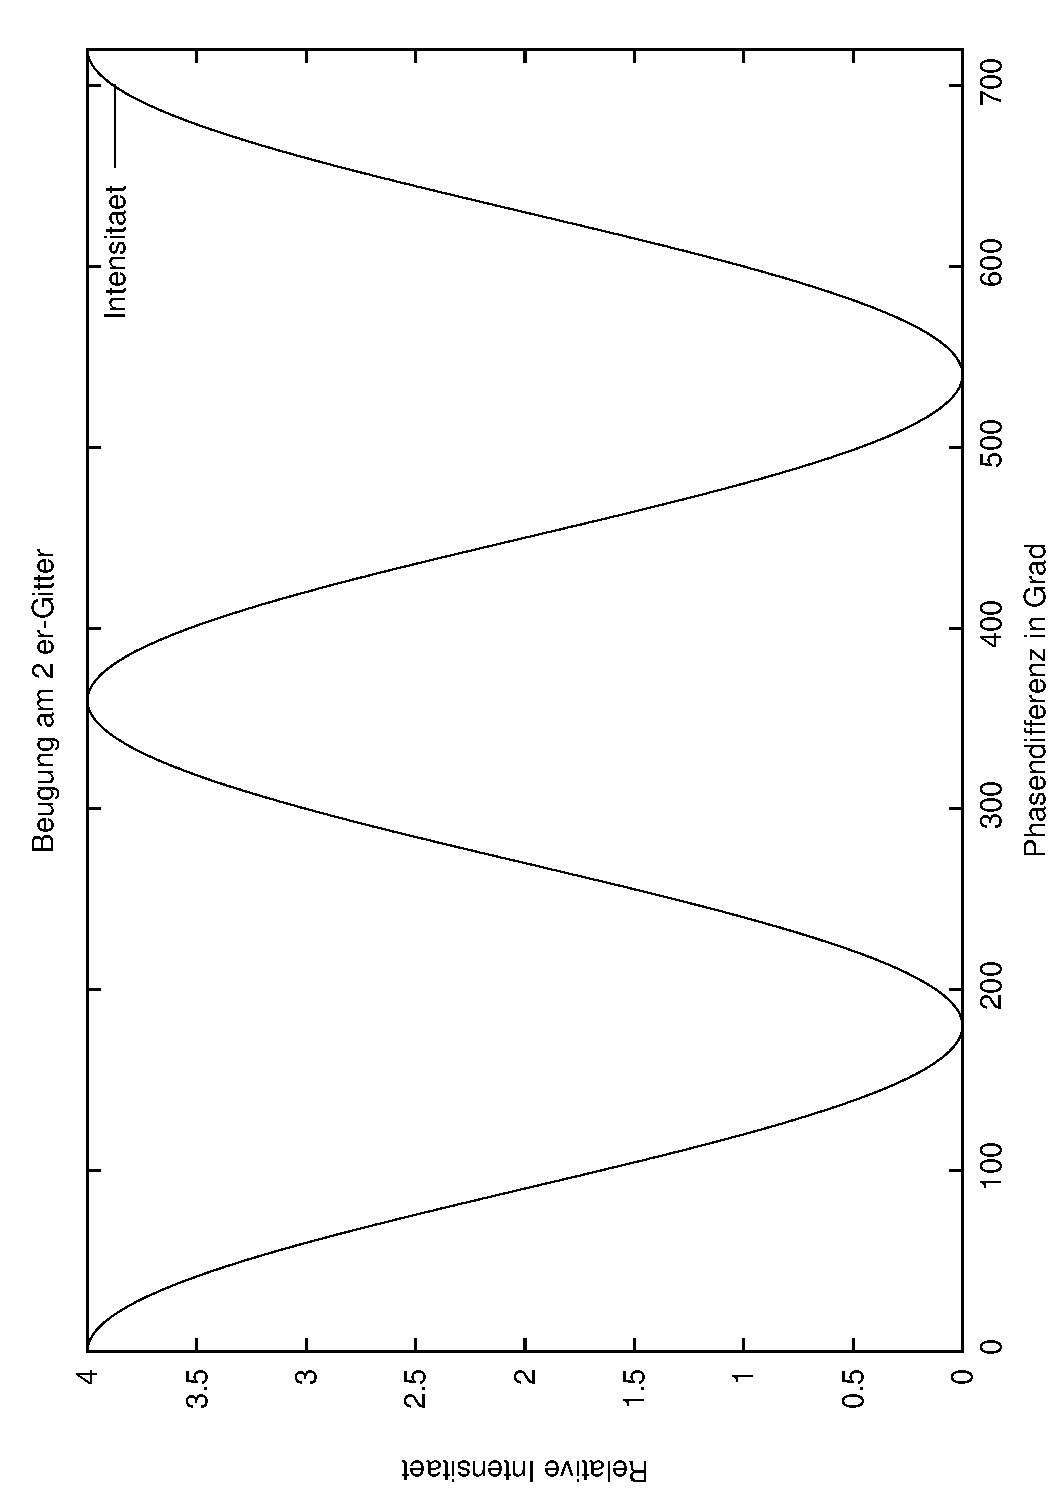
\includegraphics[width=0.43\textwidth,angle=-90]{mat/Intensitaet_doppelspalt}\label{img_intensitaet_doppelspalt}}
   
   \subfigure[Intensitätsverteilung bei Beugung am Einzelspalt (Spaltbreite 3000 nm, Wellenlänge 440 nm)]{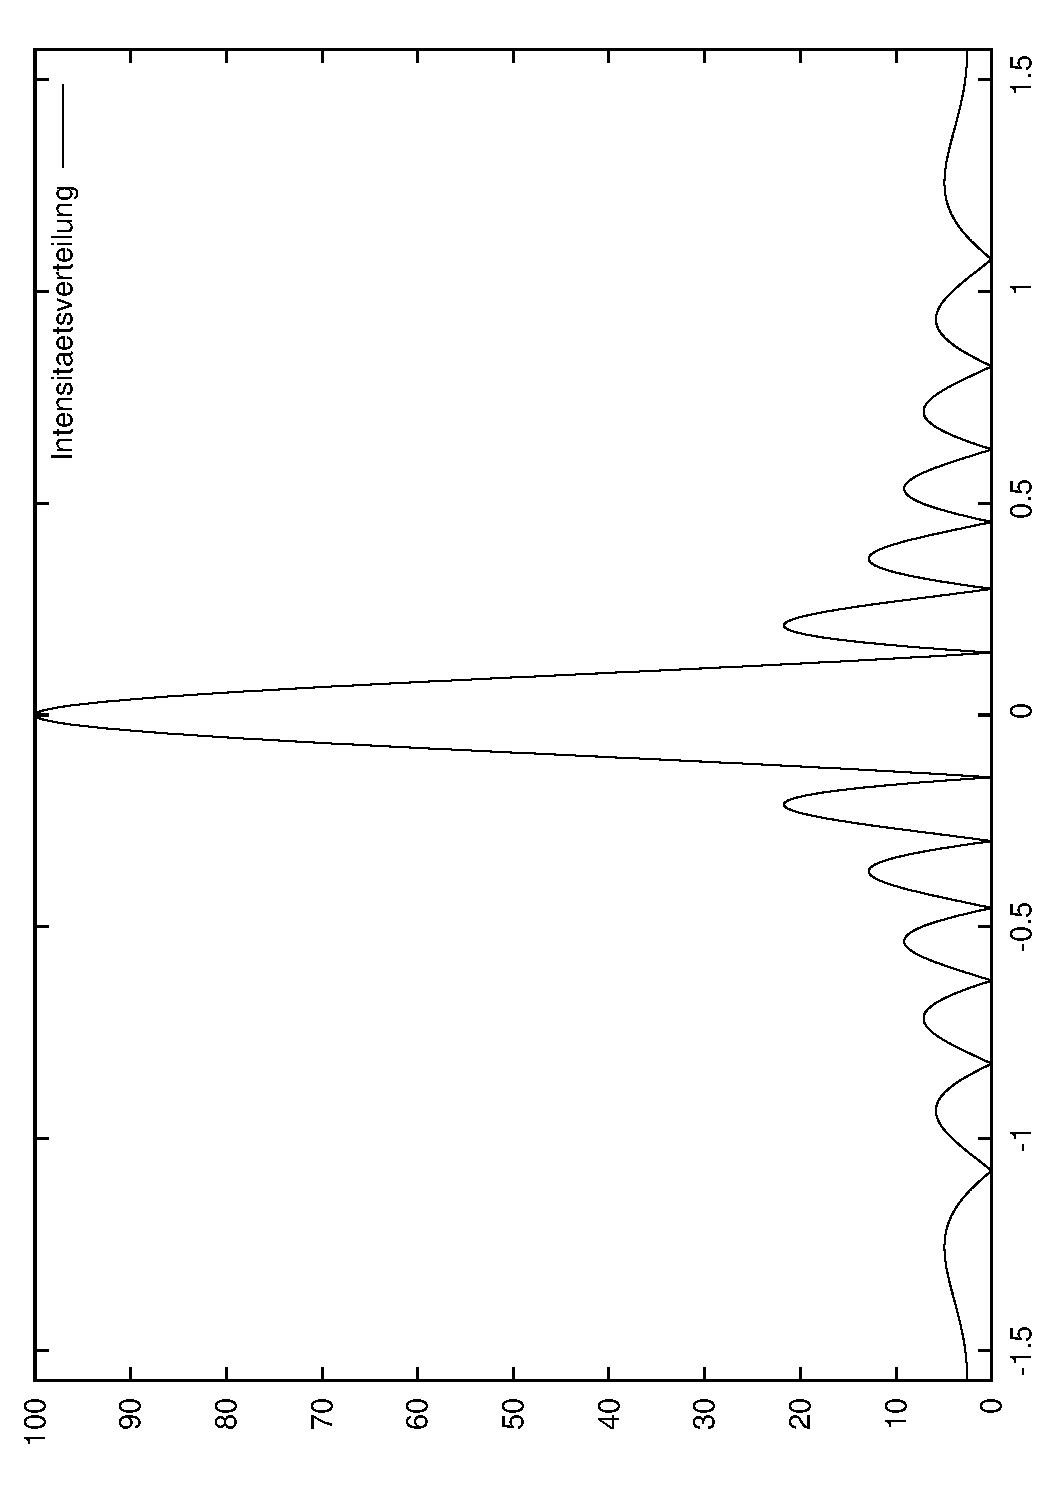
\includegraphics[width=0.43\textwidth,angle=-90]{mat/intensitaet_einzelspalt}\label{img_intensitaet_einzelspalt}}
   
   \subfigure[Intensitätsverteilung bei Beugung am Gitter bei 10 Spalten -- theoretisch!]{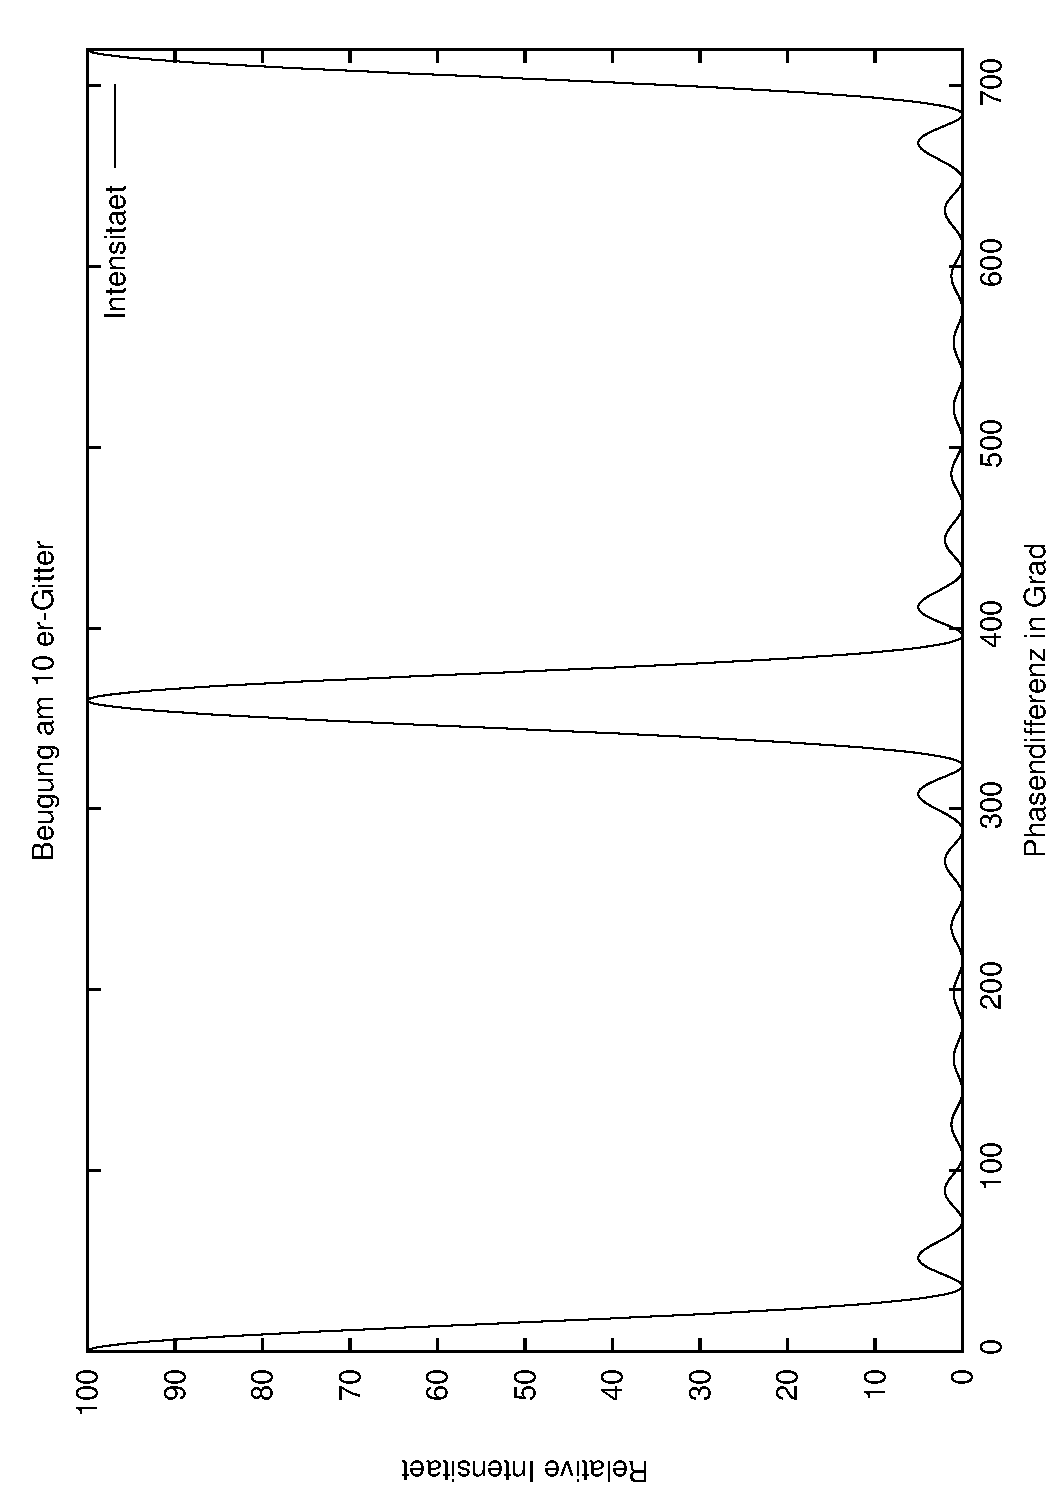
\includegraphics[width=0.43\textwidth,angle=-90]{mat/Intensitaet_zehnerspalt}\label{img_intensitaet_zehnerspalt}}
   
  
   \caption{Diverse Intensitätsverteilungen}
     
\end{figure}



		\section{\textsc{Fraunhofer}-Näherung} 
\index{Fraunhofer-Näherung!Erste}Gilt außerdem bei der Beugung am Doppelspalt
\begin{equation}
a \gg g\\
 	\label{eq_aggg}
 \end{equation}
 \begin{equation}
a \gg d_k
 	\label{eq_aggdk}
\end{equation}
so kann man sich einigen Rechenaufwand sparen. Durch Formel \ref{eq_aggg} ist nämlich der Winkel \(\alpha_k\) nicht nur unter der Linie vom Punkt zwischen den Spalten zum Punkt auf den Leuchtschirm und der Horizontalen zu finden sondern auch näherungsweise zwischen den beiden Lichtstrahlen und einer gedachten Waagerechten. Außerdem sind die beiden Lichtstrahlen dadurch praktisch parallel und (nur) deswegen kann man den Winkel \(\alpha_k\) direkt an den Spalten wiederfinden (S. Skizze). Dadurch ergibt sich ein ähnliches Dreieck\footnote{Der Winkel \(\alpha_k\) und ein rechter Winkel findet sich sowohl in den kleinen Dreieck am Doppelspalt (in der Skizze teilweise. fein gestrichelt und fett) als auch in dem Dreieck, mit dem \(\alpha_k\) bestimmt wird (in der Skizze gestrichelt).} und so kann man hier auch den Gangunterschied \(\delta\) wiederfinden (in der Skizze fett). Dadurch ergibt sich
\begin{equation}
 	\delta = g \cdot sin(\alpha_k)
 		\label{eq_gangunterschied_doppelspalt}
\end{equation}
Je nachdem, ob man einen hellen oder einen dunklen Punkt in Z betrachtet, nimmt man eine der beiden Bedingungen aus Formel \ref{eq_bedingungen_konstruktiveinterferenz} (heller Punkt) oder \ref{eq_bedingungen_destruktiveinterferenz} (dunkler Punkt) an.\footnote{Der Wert für \(k\) entspricht dabei der \emph{Ordnung} des Minimums bzw. Maximums.} 

\index{Fraunhofer-Näherung!Zweite}Bei geraden Schirmen kann man nun noch weiter vereinfachen. Der Abstand \(d_k\) ist über den geometrischen Zusammenhang
\begin{equation}
 	\frac{d_k}{a} = tan(\alpha_k) \Rightarrow d_k = a \cdot tan(\alpha_k)
 		\label{eq_doppelspalttangens}
\end{equation}
gegeben. Für \emph{sehr kleine} Winkel \(\alpha_k\) gilt
\begin{equation}
 	sin(\alpha_k) \approx \alpha_k \approx tan(\alpha_k)
 		\label{eq_winkelnaehrung}
\end{equation}
Und diese kleinen Winkel werden erreicht, wenn Formel \ref{eq_aggdk} gilt. Tut sie das \emph{nicht}, so ist diese zweite Vereinfachung nicht zulässig. Bei der Untersuchung von Lichtwellen ist dies aber normalerweise der Fall und so kann man Formel \ref{eq_gangunterschied_doppelspalt}, Formel \ref{eq_doppelspalttangens} und Formel \ref{eq_winkelnaehrung} mit den Bedingungen aus Formel \ref{eq_bedingungen_konstruktiveinterferenz} bzw. \ref{eq_bedingungen_destruktiveinterferenz} kombinieren:

Für einen maximal hellen Punkt Z bzw. ein Maximum \(k\). Ordnung gilt näherungsweise
\begin{equation}
 \delta = g \cdot \frac{d_k}{a} = k \cdot \lambda ~~~ k = (0; 1; 2; 3; \ldots)
 \label{eq_fraunhoferII_max}
\end{equation}
und dementsprechend gilt für einen dunklen Punkt Z bzw. ein Minimum \(k\). Ordnung
\begin{equation}
 \delta = g \cdot \frac{d_k}{a} = k \cdot \lambda - \frac{\lambda}{2} ~~~ k = (1; 2; 3; \ldots)
 \label{eq_fraunhoferII_min}
\end{equation}
Es ist dabei logisch, dass der größte, zu erreichende Gangunterschied \(\delta_{max} = g\) beträgt\footnote{Das wäre, wenn die Elementarwelle in senkrechter Richtung zur Doppelspaltebene betrachtet wird.}. Somit kann man sagen, dass bei der Wellenlänge \(\lambda\) aufgrund der Beziehung aus Gleichung \ref{eq_fraunhoferII_max} maximal
\begin{equation}
   k_{max} = \frac{g}{\lambda}
\end{equation}
Maxima auftreten können und aufgrund der Beziehung aus \ref{eq_fraunhoferII_min} maximal
\begin{equation}
   k_{max} = \frac{g}{\lambda} + \frac{1}{2}
\end{equation}
Minima.




 



\begin{figure}
 \centering
 \includegraphics[width=0.7\textwidth]{mat/beugung_aufbau01}
 	\caption{Skizze zum Versuchsaufbau zur \emph{Beugung am Doppelspalt}}
 		\label{img_beugungamdoppelspalt}
\end{figure}











	\section{Interferenz am Einzelspalt}
	\label{kap_interferenz_einzelspalt}
	
\index{Beugung!Einzelspalt}\index{Interferenz}Fällt eine Welle auf einen einfachen Spalt, so geschieht auch hier Interferenz. Ist der Spalt (Spaltbreite \(c\)) breit genug \(c \gg \lambda\), so geschieht diese Interferenz nur in den äußeren Randbereichen. Ist der Spalt jedoch schmal genug (\(c > \lambda\)), so ergibt sich ein richtiges Interferenzbild, wie es in Abbildung \ref{img_intensitaet_einzelspalt} auf Seite \pageref{img_intensitaet_einzelspalt} dargestellt ist.

Dieses Phenomän kann man folgendermaßen erklären (siehe dazu Abbildung \ref{img_aufbau_beugung_mehrfachspalt} auf Seite \pageref{img_aufbau_beugung_mehrfachspalt}): Das Licht das von dem Einzelspalt ausgeht, besteht aus einer Vielzahl \(n\) von Elementarwellen. Jede einzelne hat einen sehr kleinen Abstand \(g\) von ihrem Nachbarn und diese Wellen interferieren.

Der Gesamtgangunterschied für das "`Lichtbündel"' \(\delta_g\) ist dabei gemäß Formel \ref{eq_gangunterschied_doppelspalt} zu bestimmen. Der Gangunterschied zweier benachbarter Wellen \(\delta_e\) beträgt somit 
\begin{equation}
   \delta_e = \frac{sin(\alpha) \cdot c}{n}
\end{equation}
Nun greift man sich zwei Licht"`strahlen"' heraus. Ihre Ursprünge haben in der Spaltebene den Abstand \(s\)
\begin{equation}
   s = \frac{\lambda}{2 \cdot sin(\alpha)}
   \label{eq_einzelspalt_s}
\end{equation}
und somit haben sie den Gangunterschied \(\delta = \frac{\lambda}{2}\). Nach Formel \ref{eq_bedingungen_destruktiveinterferenz} löschen sich diese beiden Wellen also aus. Ebenso löschen sich die einzelnen Nachbarwellen der jeweiligen Wellen völlig aus. Die Elementarwellen, die in der Spaltebene den Abstand \(s\) voneinander haben, löschen sich also generell aus. Somit ist der Bereich \(c_{hell}\) in der Spaltebene, in dem die Elementarwellen \emph{nicht} ausgelöscht werden, folgendermaßen berechenbar:
\begin{equation}
   c_{hell} = c - s \cdot i ~~~ i = (0; 2; 4; ...)
   \label{eq_einzelspalt_a_hell}
\end{equation}
Der Faktor \(i\) muss gerade sein, weil sich immer zwei Wellen auslöschen; eine aus dem bereich \([0;s[\), die andere aus dem Bereich \([s;2s[\). Somit ergibt sich aus Formel \ref{eq_einzelspalt_s} und Formel \ref{eq_einzelspalt_a_hell} die Folgerung, dass unter bestimmten Winkeln \(\alpha_k\) kein Licht auf einem Schirm hinter dem spalt sichtbar ist, weil sich \emph{alle} einzelnen Wellen auslöschen. Dies ist der Fall wenn \(\delta_g = \lambda \cdot k\). \(c_{hell}\) kann dabei niemals \(c_{hell} = s\)  sein.\footnote{Bei mehr als \(s\) hätten manche Wellen schon wieder Partner um sich gegenseitig auszulöschen.}

Trotzdem sind wie in Abbildung \ref{img_intensitaet_einzelspalt} nicht alle Maxima gleich hoch. Das ligt daran, dass der Anteil \(\frac{c_{hell}}{c}\) nur für \(\alpha = 0\) ~ \(1\) ergeben kann -- für alle weiteren Winkel \(\alpha\) ist er kleiner. Entscheidend für die weitere Intensitätsabnahme ist aber, dass die Intensität \(I\) vom E-Feld-Vektor abhängt:
\begin{equation}
   I \sim \vert \vec{E} \vert ^2
   \label{eq_intensitaet}
\end{equation}
Dieser Betrag des E-Feld-Vektors (\(\vert \vec{E} \vert\)) nimmt kontinuierlich ab, weil er sich aus den E-Feld-Vektoren der einzelnen Elementarwellen zusammensetzt. Die Summe dieser schließlich nimmt deswegen mit wachsenden Winkeln \(\alpha\) ab, weil die Phasendifferenz zwischen den einzelnen Vektoren wächst (Formel \ref{eq_gangunterschied_doppelspalt} und \ref{eq_zshg_phasendif_ganguntersch}). Bei der Vektoraddition ergeben sich maximale Vektoren aus einzelnen Vektoren, wenn diese alle parallel zueinander stehen. Je weniger parallel (also je größer die Phasendifferenz) desto kleiner ist das Vektoraddukt (der Vektorweg wird immer kugeliger) und desto kleiner ist die Intensität.






\begin{figure}
   \centering
   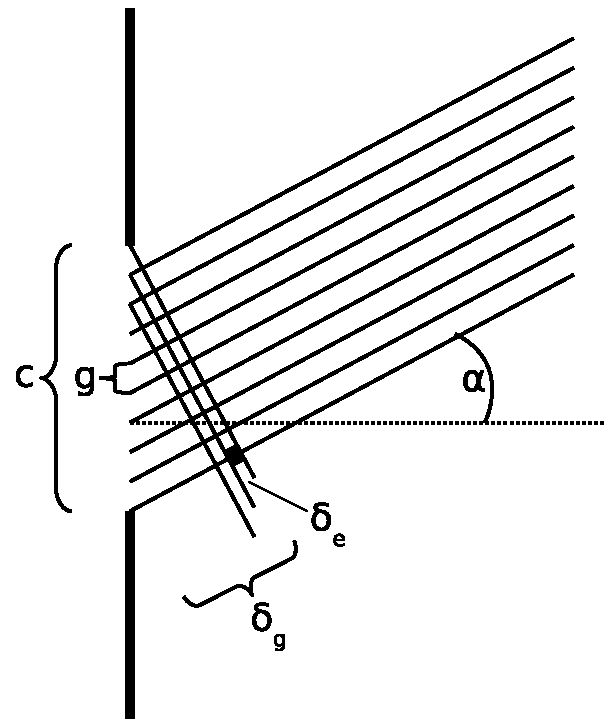
\includegraphics[width=0.5\textwidth]{mat/beugung_mehrfachspalt}
   \caption{Skizze zu Interferenz am Einzelspalt bzw. am Gitter}
   \label{img_aufbau_beugung_mehrfachspalt}
\end{figure}







	\section{Interferenz am Gitter}


\index{Beugung!Gitter}\index{Beugung!Mehrfachspalt}\index{Interferenz}Ein Gitter ist ein Mehrfachspalt. Die \textit{Gitterkonstannte} \(g\) gibt an, wie weit die Mittelpunkte zweier benachbarter Gitter auseinander liegen. Interferenz am Gitter funktioniert im Prinzip wie Interferenz am Einzelspalt, nur dass hier nicht unendlich viele Elementarwellen entstehen / interferrieren. Die Bedingungen für Minima und Maxima sind aus Kap. \ref{ss_beugung_doppelspalt} zu entnehmen. Betrachtet man Abbildung \ref{img_aufbau_beugung_mehrfachspalt}, so wird klar warum: der Gangunterschied \(\delta_e\) zwischen zwei einzelnen Spalten ist entscheidend dafür, ob die beiden Wellen einander auslöschen. Dieser ist dank der Definition der Gitterkonstante ebenso zu berechnen wie beim Doppelspalt.


Ein bedeutender Unterschied zwischen Beugung am Doppelspalt und Beutung am Gitter ist aber das entstehende Interferenzbild: Die einzelnen Maxima sind beim Gitter nämlich wesentlich weiter voneinander entfernt und außerdem schärfer. Vergleicht man Abbildung \ref{img_intensitaet_doppelspalt} und \ref{img_intensitaet_zehnerspalt} auf Seite \pageref{img_intensitaet_doppelspalt}, so ist dies ersichtlich. 

Die Erklärung für die vielen \emph{kleinen} Maxima ist dass hier die \(\vec{E}\) bei der Addition geschlossene Vektorzüge ("`Kreise"') bilden, die nichts produktives zur Intensität beitragen (siehe Formel \ref{eq_intensitaet}). Schärfer werden die Maxima dadurch, dass die Intensitäten schneller abfallen.


Für das Gitter gilt die selbe Einschränkung wie für den Doppelspalt: Die einzelnen Spalte fungieren jeweils als Einzelspalt, wodurch sich in einem realen Beugungsbild zwei verschiedene Phenomäne überlagern.







	\section{Spektrale Zerlegung}

Bisher wurde bei der Beugung nur eine einzige Farbe in Betracht gezogen ("`\textit{monochromatisches}"' Licht)\index{Monochromatisch}. Verwendet man bei einer Beugung jedoch Licht aus mehreren Farben\footnote{"`normales"', weißes Licht besteht aus vielen verschiedenen Farben}, so muss man die Maxima für die einzelnen Farben entsprechend berechnen. Es ergeben sich so in ein und dem selben Aufbau verschiedene Interferenzbilder für die verschiedenen Farben, die sich gegenseitig überlagern können.\index{Spektrale Zerlegung}








		\chapter{Brechung}

	\section{Beschreibung}

\index{Brechung}Bei der Brechung wird eine Welle beim Übergang in ein anderes Medium von seiner ursprünglichen Ausbreitungsrichtung abgelenkt. Diese Ablenkung basiert auf unterschiedlichen Ausbreitungsgeschwindigkeiten in unterschiedlichen Medien. Eine Begleiterscheinung ist die Reflexion.\index{Reflexion}

Grundsätzlich tritt Brechung bei verschiedenen Wellenformen auf, hauptsächlich spricht man jedoch im Bereich der Optik von Brechung. Im Allgemeinen sind die Angaben aber auch auf bspw. Erdbebenwellen zu beziehen.

Für den Einfallswinkel \(\alpha\) und den Ausfallswinkel \(\beta\)\index{Einfallswinkel}\index{Ausfallswinkel} -- beide gegenüber einem Lot\index{Lot} gemessen, welches senkrecht auf der Grenzfläche zwischen den Materealien steht -- gilt dabei der Zusammenhang:
\begin{equation}
   \frac{sin(\alpha)}{sin(\beta)} = \frac{n_2}{n_1} = n_{2,1} = \frac{c_1}{c_2}
   \label{eq_brechungsgesetz}
\end{equation}
Dabei sind \(n_M\) \emph{absolute} Brechzahlen\index{Brechzahlen}\index{Absolute Brechzahl} der Materealien \(M\): Das Verhältnis der Vakuumlichtgeschwindigkeit \(c_0\) zur Ausbreitungsgeschwindigkeit im Medium \(c_M\):
\begin{equation}
   n_M = \frac{c_0}{c_M}
   \label{eq_absoluter_brechungsindex}
\end{equation}
 \(n_{2,1}\) wird als \textit{relativer} Brechungsindex für den Übergang von Material 2 nach Material 1 bezeichnet.

Ist \(n_2 > n_1\) so spricht man bei \(M_2\) vom optisch \textit{dichteren}\index{Optisch dichter bzw. dünner} und bei \(M_1\) vom optisch \textit{dünneren} Medium. Im dichteren Medium pflanzt sich eine Welle langsamer fort und dementsprechend wird die Wellenlänge beim Übergang in ein optisch dichteres Medium kürzer.
 



	\section{\textsc{Huygens}}

\index{Huygen'sches Prinzip}Mit dem \textsc{Huygens}'schen Prinzip lassen sich sowohl Brechung als auch Reflexion anschaulich darstellen: Bei der Brechung breiten sich die von der Wellenfront am Materialübergang entstehenden Elementarwellen im optisch dichteren Medium langsamer aus, überlagern sich dann aber wieder zu einer Wellenfront. Verfolgt man parallel zu den sich im optisch dichteren Medium ausbreitenden Elementarwellen die, die sich weiterhin im optisch dünneren Medium ausbreiten, so erkennt man hier, dass sich diese Wellen zu einer reflektierten Wellenfront überlagern.


	\section{Totalreflexion}

\index{Totalreflexion}Allgemein gilt, dass der Lichtweg umkehrbar ist. Wird ein Lichtstrahl also in ein optisch dicheres Medium gebrochen und dort genau senkrecht reflektiert, so nimmt es genau den Weg, den es gekommen ist, wieder zurück. 

Fällt Licht jedoch unter einem Winkel von einem optisch dichteren Medium in ein optisch dünneres, sodass der Austrittswinkel rein rechnerisch über \(90^o\) liegen würde, so tritt \textit{Totalreflexion} auf. Der Einfallswinkel, bei dem dies stattfindet, wird als \textit{Grenzwinkel} \(\alpha_{grenz}\) bezeichnet.\index{Grenzwinkel} Normalerweise wird stets ein kleiner Anteil der Welle beim Übertritt in ein anders Medium reflektiert und dieser Anteil wächst, je größer der Einfallswinkel wird. Bei Totalreflexion wird die komplette Welle reflektiert und ins opitsch dichtere Medium zurückgeworfen.



	\section{Übergang dicht -- dichter}

Beim Übergang einer Welle von einem optisch dünneren in ein optisch dichteres Medium wird die Welle stets mit Phasensprung \(\Delta \varphi = \pi\) reflektiert, nur beim Übergang vom optisch dichteren ins optisch dünnere Medium erfolgt die Reflexion ohne Phasensprung.\index{Phasensprung}



	\section{Dispersion}

Als \textit{Dispersion}\index{Dispersion} bezeichnet man die Abhängigkeit des Brechungsindexes eines Materials von der Wellenlänge bzw. Frequenz des einfallenden Lichts. Je kurzwelliger bzw. hochfrequenter eine Welle ist, desto stärker wird sie gebrochen und desto größer ist folglich ihr Brechungsindex. Diese Eigenschaft macht man sich zunutze, um ein Spektrum zu erzeugen: In einem Prisma wird violettes Licht stärker gebrochen als rotes. Leuchtet man mit einem eng begrenzten weißen Lichtbündel auf ein Prisma, so erhält man dahinter ein (soweit die Farben im Weiß vorhanden waren) kontinuierliches Spektrum.





	\section{Spektrenvergleich}

\index{Spektrale Zerlegung!Vergleich Doppelspalt und Prisma}In Tabelle \ref{tab_spektrenvergleich} auf S. \pageref{tab_spektrenvergleich} werden wichtige Eigenschaften eines Spektrums vom Doppelspalt mit denen vom Prismenspektrum verglichen.

\begin{table}[h]
	\centering
	
   \begin{tabular}{l | l | l}
      ~ & \textbf{\textit{Gitter}} & \textbf{\textit{Prisma}} \\
      \hline
      \textit{Ursache} & Beugung durch Interferenz & Dispersion bei Brechung \\
      \textit{Farbanordnung} & Rot wird weiter weg abgelenkt & Blau wird stärker gebrochen\\
      \textit{Kontinuität} & mehrere Spektren neben- und übereinander & kontinuierliches Spektrum \\
      \textit{Anzahl} & mehrere Maxima je Farbe (möglich) & Jede Farbe nur einmal \\      
   \end{tabular}
\caption{Verglich der spektralen Zerlegung von Licht nach Beugung am Gitter und Brechung am Prisma}
\label{tab_spektrenvergleich}
\end{table}






		\chapter{Polarisation}

Als \textit{linear polarisiert}\index{Polarisation}\index{Linear polarisiert} bezeichnet man Licht, dessen E-Feld-Vektoren alle in einer Ebene schwingen. Somit lassen sich logischerweise nur Quer- bzw. Transversalwellen polarisieren.


	\section{EMW an Gitterstäben}

Eine linear polarisierte Elektromagnetische Welle kann ein metallenes Gitter nur dann passieren, wenn ihr \(\vec{E}\) senkrecht zu den Gitterstangen schwingt. Danntabular werden die Elektronen in den Stäben nämlich nicht zu starken Schwingungen angeregt (bzw. sie können aus Platzgründen nicht schwingen). Ist die Polarisationsebene jedoch parallel zu den Gitterstäben, so wird in den Stäben eine Schwingung erzwungen. Diese sorgt über ein kompliziertes Interferenzverfahren dafür, dass die Elektromagnetische Welle ausgelöscht wird.

Trifft eine solche Welle schräg auf ein Gitter, so kann stets nur der Teil -- also die Komponente -- das Gitter passieren, die senkrecht zu den Gitterstäben steht. Auf diese Weise wird die Polarisationsebene des Lichts geändert: Vorher war sie schräg zu den Gitterstäben, jetzt die "`überlebende"' Komponenten senkrecht zum Gitter ausgerichtet. Natürlich hat die Welle dabei an Intensität eingebüßt. Trifft eine Welle unter dem Winkel \(\alpha\) auf ein Gitter (\(\alpha\) bezeichnet den Winkel der Polarisationsebene mit dem Horizont bei lotrechten Gitterstäben), so kann nur ein Anteil \( \vert \vec{E}_a \vert \) weiterlaufen:
\begin{equation}
   \vert \vec{E}_a \vert = \vert \vec{E}_0 \vert \cdot sin(\alpha)
\end{equation}
Sind zwei Polarisationsfilter\index{Polarisationsfilter} parallel hintereinander aufgestellt mit senkrechten Polarisationsebenen, so dass normalerweise kein Licht hindurchgelangen könnte, so kann ein Anteil des Lichts die Filter passieren, wenn man noch einen dritten zwischen die beiden Filter stellt, dessen Polarisationsebene von denen der beiden anderen abweicht. Von einer Welle, die den ersten Filter passiert hat (\(\vert \vec{E}_a \vert\)), gelangt dann der Anteil \(\vert \vec{E}_d \vert\) durch den Aufbau, wenn der neue Polarisationsfilter mit dem Winkel \(\beta\) zum ersten steht:
\begin{equation}
   \vert \vec{E}_d \vert\ = \vert \vec{E}_a \vert \cdot \frac{1}{2} \cdot sin(2 \cdot \beta)
\end{equation}





	\section{Polarisation bei Brechungsvorgängen}

\index{Polarisation!Durch Brechung}Bei den folgenden Erklärungen sollte bedacht werden, dass eine Elektromagnetische Welle stets die Elektronen in ihrer Umgebung zu Schwingung anregt -- und zwar in Richtung ihres \(\vec{E}\). Fasst man die schwingenden Elektronen als Dipol auf, so kann dieser Dipol keine Welle parallel seiner Schwingungsrichtung / Längsachse ausstrahlen, sondern nur senkrecht dazu. Bei unpolarisiertem Licht schwingen die Elektronen also in alle Richtungen senkrecht zur Ausrbeitungsrichtung eines Lichtbündels.

	
		\subsection{Streuung}
		
\index{Polarisation!Durch Streuung}Wird ein Lichtbündel gestreut und ändert so seine Ausbreitungsrichtung um \(90^o\), kommen nur Elektronen in Frage, die sowohl senkrecht zur ehemaligen als auch zur neuen Ausbreitungsrichtung schwingen. Da nur diese eine Richtung in Frage kommt, schwingt das gestreute Licht auch nur in dieser Richtung -- ist also linear polarisiert.


		\subsection{\textsc{Brewster}-Winkel}

\index{Brewster-Winkel}\index{Polarisation!Brewster-Winkel}Stehen bei einer Brechung die Ausbreitungsrichtungen von reflektiertem und gebrochenem Lichtstrahl genau senkrecht aufeinander, so ist das reflektierte Licht völlig linear polarisiert. Es kommt nämlich auch hier nur eine einzige mögliche Richtung in Frage, in der die Elektronen Schwingen könnten, um einerseits noch in der vom gebrochenen Licht erzeugten Ebene zu schwingen und andererseits senkrecht zur neuen Ausbreitungsrichtung zu schwingen. 








		\chapter{Erdbeben - Kurzübersicht}


\index{Erdbeben}Durch tektonische Vorgänge können sich in der Erde Spannungen bilden, die sich dann bei einem Erdbeben lösen, wenn die Gesteinsschichten wegschnellen. Die Erde in der Umgebung des Epizentrums wird zum Mitschwingen angeregt. Ein Erdbebenzentrum liegt in \(30\) bis \(800 km\) Tiefe. Longitudinalwellen breiten sich mit \(c \approx 6 \frac{km}{h}\) in allen Richtungen aus, Transversalwellen folgen mit \(c \approx 3 \frac{km}{h}\), wobei diese sich nicht im flüssigen Erdkern weiter fortbewegen können. Große Zerstörungen verursachen dabei auch die von diesen beiden Wellen angeregten \textit{Oberflächenwellen}\index{Oberflächenwellen} an der Erdoberfläche mit starken Horizontalbeschleunigungen, die mit Frequenzen zwischen \(f \in [1;30] ~ Hz\) schwingen. Gebäude versucht man deshalb auch so zu bauen, dass sie in diesem Frequenzbereich keine Eigenfrequenz aufweisen.









		\chapter{Schallwellen}

\index{Schallwellen}Bei Schallwellen handelt es sich um \emph{Longitudinalwellen}\footnote{In Festkörpern können sie sich auch als Transversalwellen fortpflanzen.}. Hierbei schwingen die Massenteilchen längs der Ausbreitungsrichtung um eine Ruhelage. Dadurch entstehen Regionen erhöhten und verminderten Drucks. An Stellen maximalen \textit{(a)} und minimalen \textit{(b)} Drucks sind die Teilchen dabei in Ruhe, wobei ihre Schnelle \textit{(a)} in Richtung bzw. \textit{(b)} entgegen der Ausbreitungsrichtung wirkt.

Was in den vorangegangenen Kapiteln gesagt wurde, stimmt für Schallwellen auch weiterhin. Hier muss man allerdings bedenken, dass man Bei Schallwellen nicht eindeutig von \emph{Wellenbäuchen} sprechen kann. Wo nämlich ein \emph{Druck}bauch ist, sitzt gleichzeitig ein \emph{Schnellen}knoten.\footnote{Was man mit einem Mikrophon messen kann sind die Veränderungen des Luftdrucks}.\index{Druckbauch}\index{Schnellenbauch}

Die Ausbreitungsgeschwindigkeit \(c\) des Schallwellen ist dabei abhängig vom Ausbreitungsmedium\footnote{Luft: ca. \(340 \frac{m}{s}\); Wasser: ca. \(1485 \frac{m}{s}\); Eisen: ca. \(5200 \frac{m}{s}\)} und von der Temperatur, wobei der Luftdruck die Schallgeschwindigkeit nicht beeinflusst.


\subsubsection{Reflexionen, Überlagerungen \& Co}

\index{Reflexion}Schallwellen können an festen Gegenständen - wie bspw. Wänden - reflektiert werden. Dabei bildet sich an dem festen Gegenstand ein Schnellenknoten bzw. Druckbauch. In einem begrenzten Hohlkörper kann darüber hinaus noch zusätzlich Reflektion an einem offenen Ende geschehen; dann liegt am Offenen Ende ein Bewegungsbauch. Die Reflektion an einem festen Gegenstand entspricht dabei der an einem festen Ende, Reflektion an einem offenen Ende entspricht dabei der am losen Ende des Wellenträgers.









		\chapter{Elektromagnetische Wellen}


		\section{Dipol}

Lässt man in einem Schwingkreis\index{Schwingkreis} Ladungen schwingen, so wird gleichzeitig eine elektromagnetische Welle\index{Elektromagnetische Welle} emittiert.\footnote{Das bemerkt man bspw. wenn man einen Schwingkreis (mit richtiger Kapazität \(C\) und Induktivität \(L\)) in der Nähe eines Radios schließt - es wird im Radio ein Knacken zu hören sein.} Aus den \textsc{Thomson}'schen Schwingungsgleichungen ergibt sich dabei für die Frequenz, mit der der Schwingkreis schwingt und damit auch seine elektromagnetische Welle:
\begin{equation}
 	f_0 = \frac{1}{2 \cdot \pi \cdot \sqrt{C \cdot L}}
 	\label{freq_emw}
\end{equation}
Es handelt sich dabei um die \emph{Eigenfrequenz}\index{Eigenfrequenz} des Schwingkreises. Es ist also nicht alleine die Frequenz, bei der er seine elektromagnetische Strahlung aussendet, sondern auch die Frequenz, mit der er angeregt werden kann, wobei sich maximale Resonanz ergibt.




		\section{\textsc{Hertz}'scher Dipol}

\index{Hertz'scher Dipol}Um einen Dipol mit hohen Frequenzen anregen zu können, versucht man also die Werte für \(C\) und \(L\) möglichst \emph{klein} zu bekommen. Das gelingt, indem man einen Kondensator mit möglichst Breitem Plattenabstand und kleinen Plattenflächen nebst einer Spule mit wenig Querschnittsfläche, geringer Windungszahl und kleiner Länge verwendet. Verändert man einen Schwingkreis konsequent nach diesen Richtlinien, erhält man einen  \emph{\textsc{Hertz}'schen Dipol}. Er besteht aus einem schlichten Draht. Dabei übernehmen die Drahtenden die Funktionen der Kondensatorplatten und der Draht selbst fungiert als Spule.






		\section{Erregung des \textsc{Hertz}'schen Dipols durch EM Wellen}

Auf einem Empfangsdipol\index{Empfangsdipol} kann sich eine stehende Welle bilden, wenn seine Länge \(L\) mit Formel \ref{eq_2lose} über\-ein\-stimmt. Platziert man einen Verbraucher auf dem \textsc{Hertz}'schen Dipol, so muss man beachten, dass sich an manchen Stellen Strom- und an manchen Stellen Ladungsknoten bilden.\footnote{Ein Glimmlämpchen kann man so nicht in der Mitte eines Dipols der Länge \(L = \lambda\) zum Leuchten bringen, weil sich hier ein Stromknoten herausbildet und das Lämpchen Strom zum Leuchten bräuchte.}

An den Dipolenden ergeben sich Ladungsbäuche\index{Ladungsbauch}, weil sich hier schließlich die \textit{Kondensatorplatten} befinden, auf denen sich die Ladung komplett sammelt, wenn die komplette Energie der Schwingung in elektrischer Feldenergie vorliegt. Hat man einen Dipol, der länger ist als \(\frac{\lambda}{2}\), so ergeben sich auf der Länge des Dipols mehrere Stellen, an denen die Ladung sich zu Maxima 'sammelt' (s. Abb. \ref{img_Ix-Qx} auf S. \pageref{img_Ix-Qx})

Es ist dabei aber entscheidend, in welchem \emph{Medium} sich der Dipol befindet (\(\rightarrow\) Kap. \ref{ss_Ausbreitungsgeschwindigkeit} auf S. \pageref{ss_Ausbreitungsgeschwindigkeit}).


\begin{figure}
\centering
 \subfigure[I-x-Diagramm, \(L = \lambda\), \(t = 0\)]{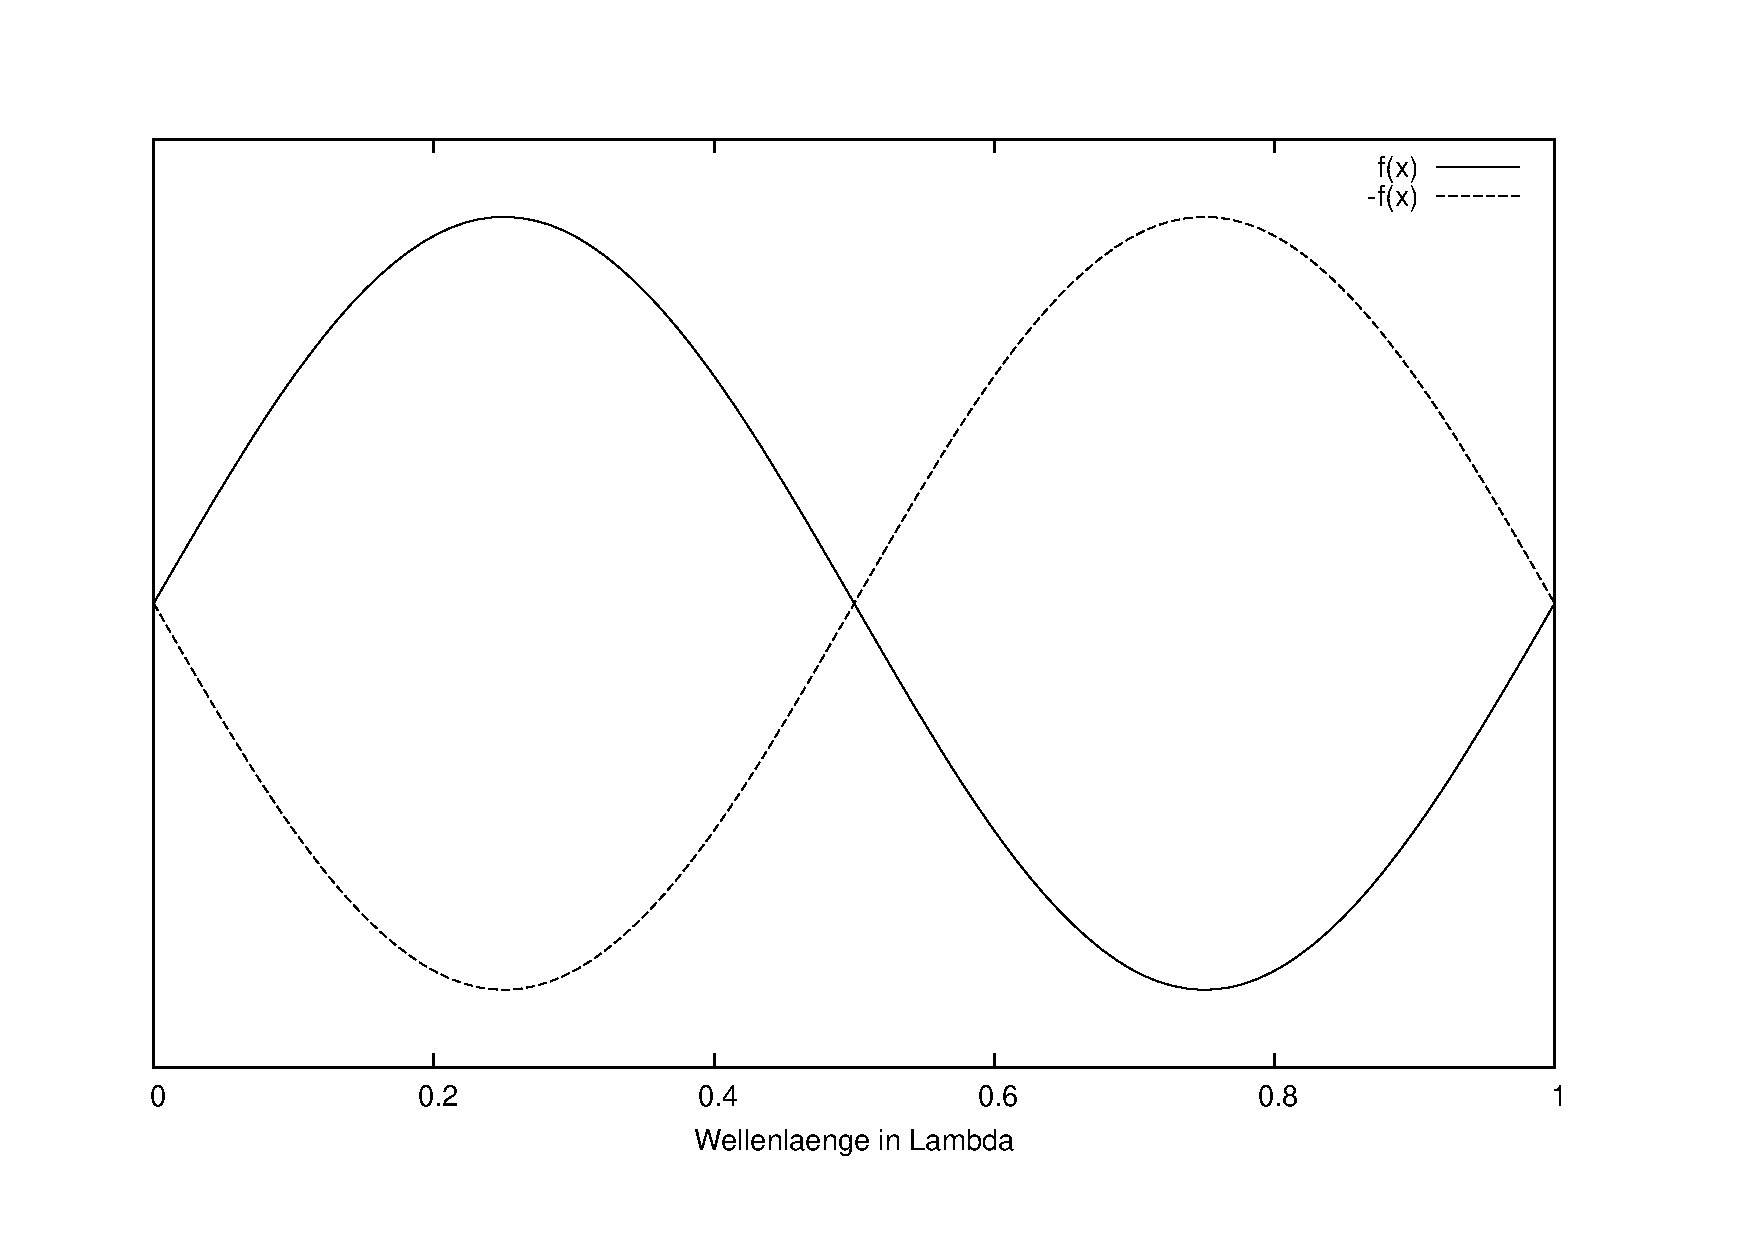
\includegraphics[width=0.4\textwidth]{mat/I10}}
 \subfigure[I-x-Diagramm, \(L = \frac{\lambda}{2}\), \(t = 0\)]{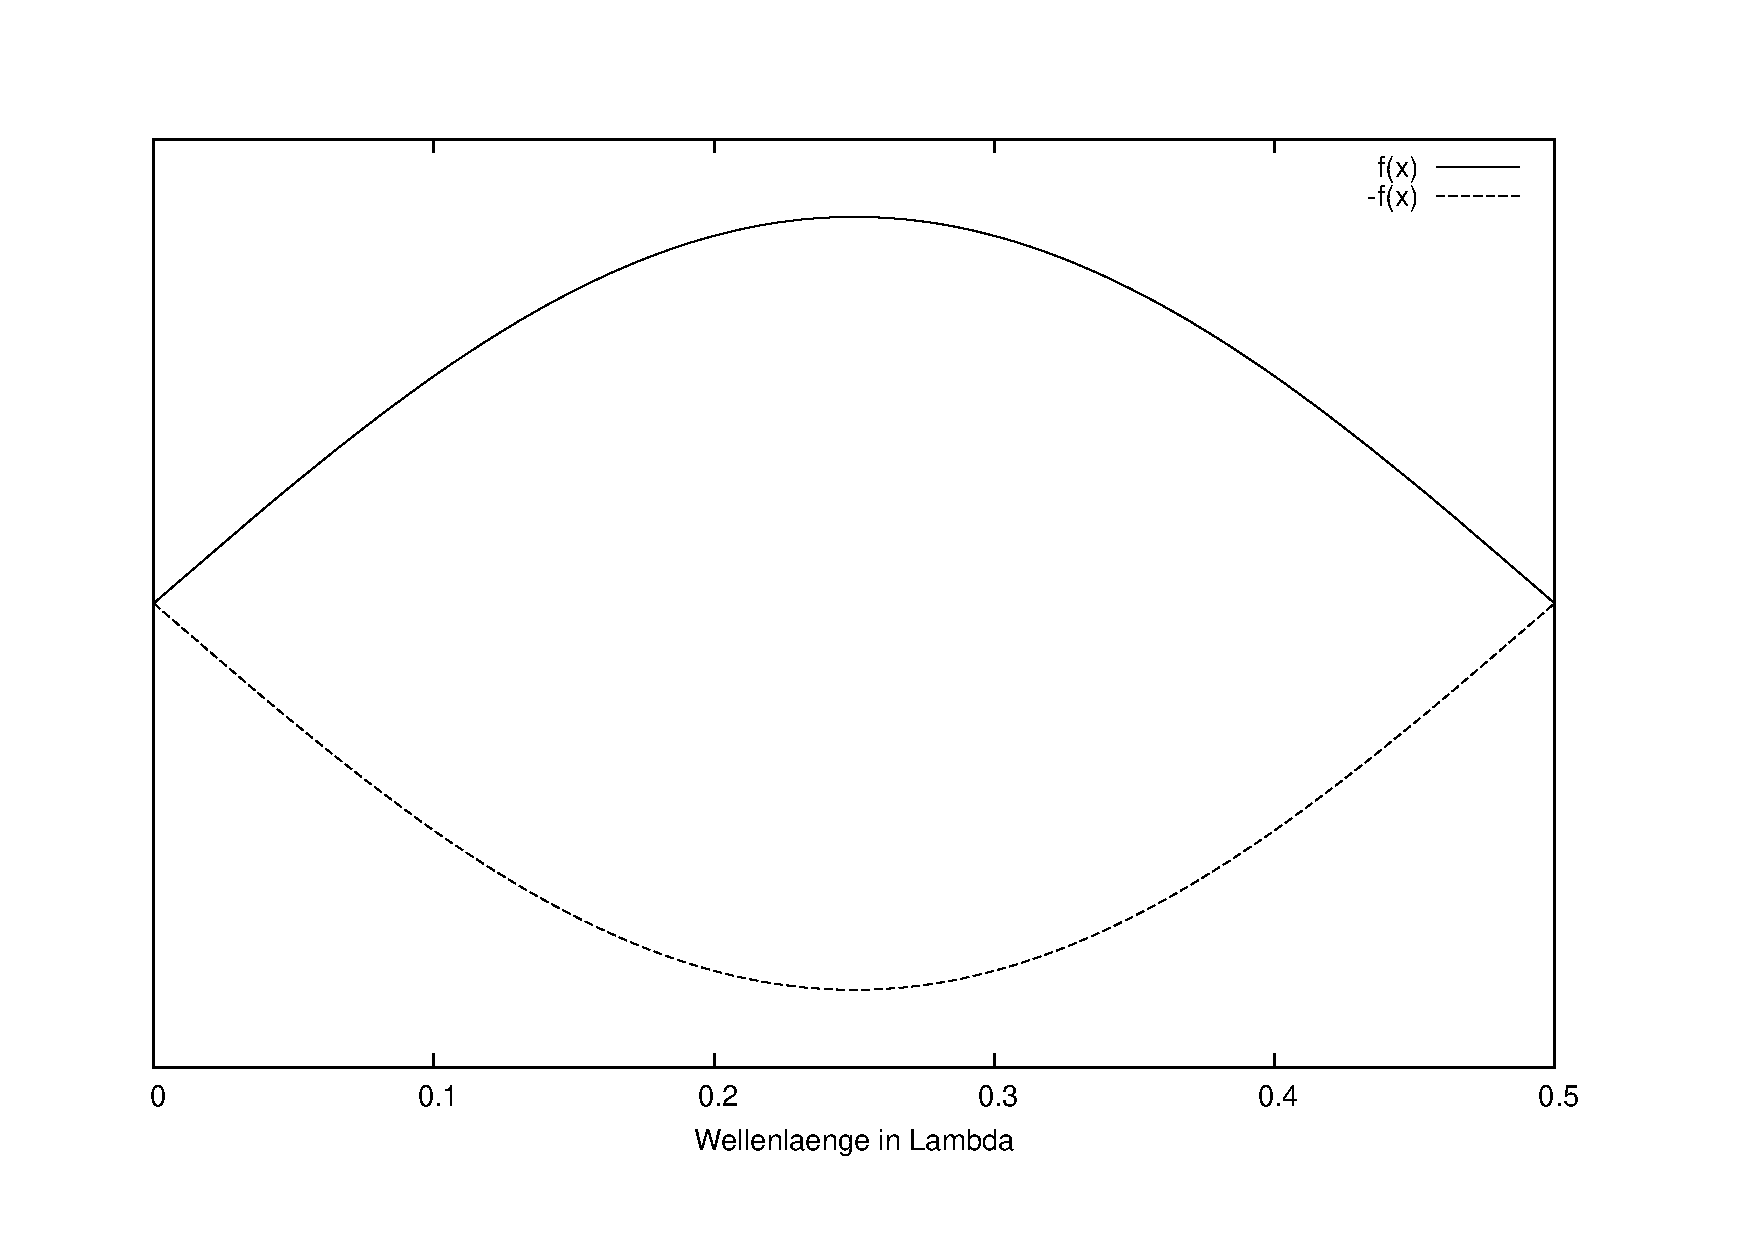
\includegraphics[width=0.4\textwidth]{mat/I05}}
 \subfigure[Q-x-Diagramm, \(L = \lambda\), \(t = \frac{T}{4}\)]{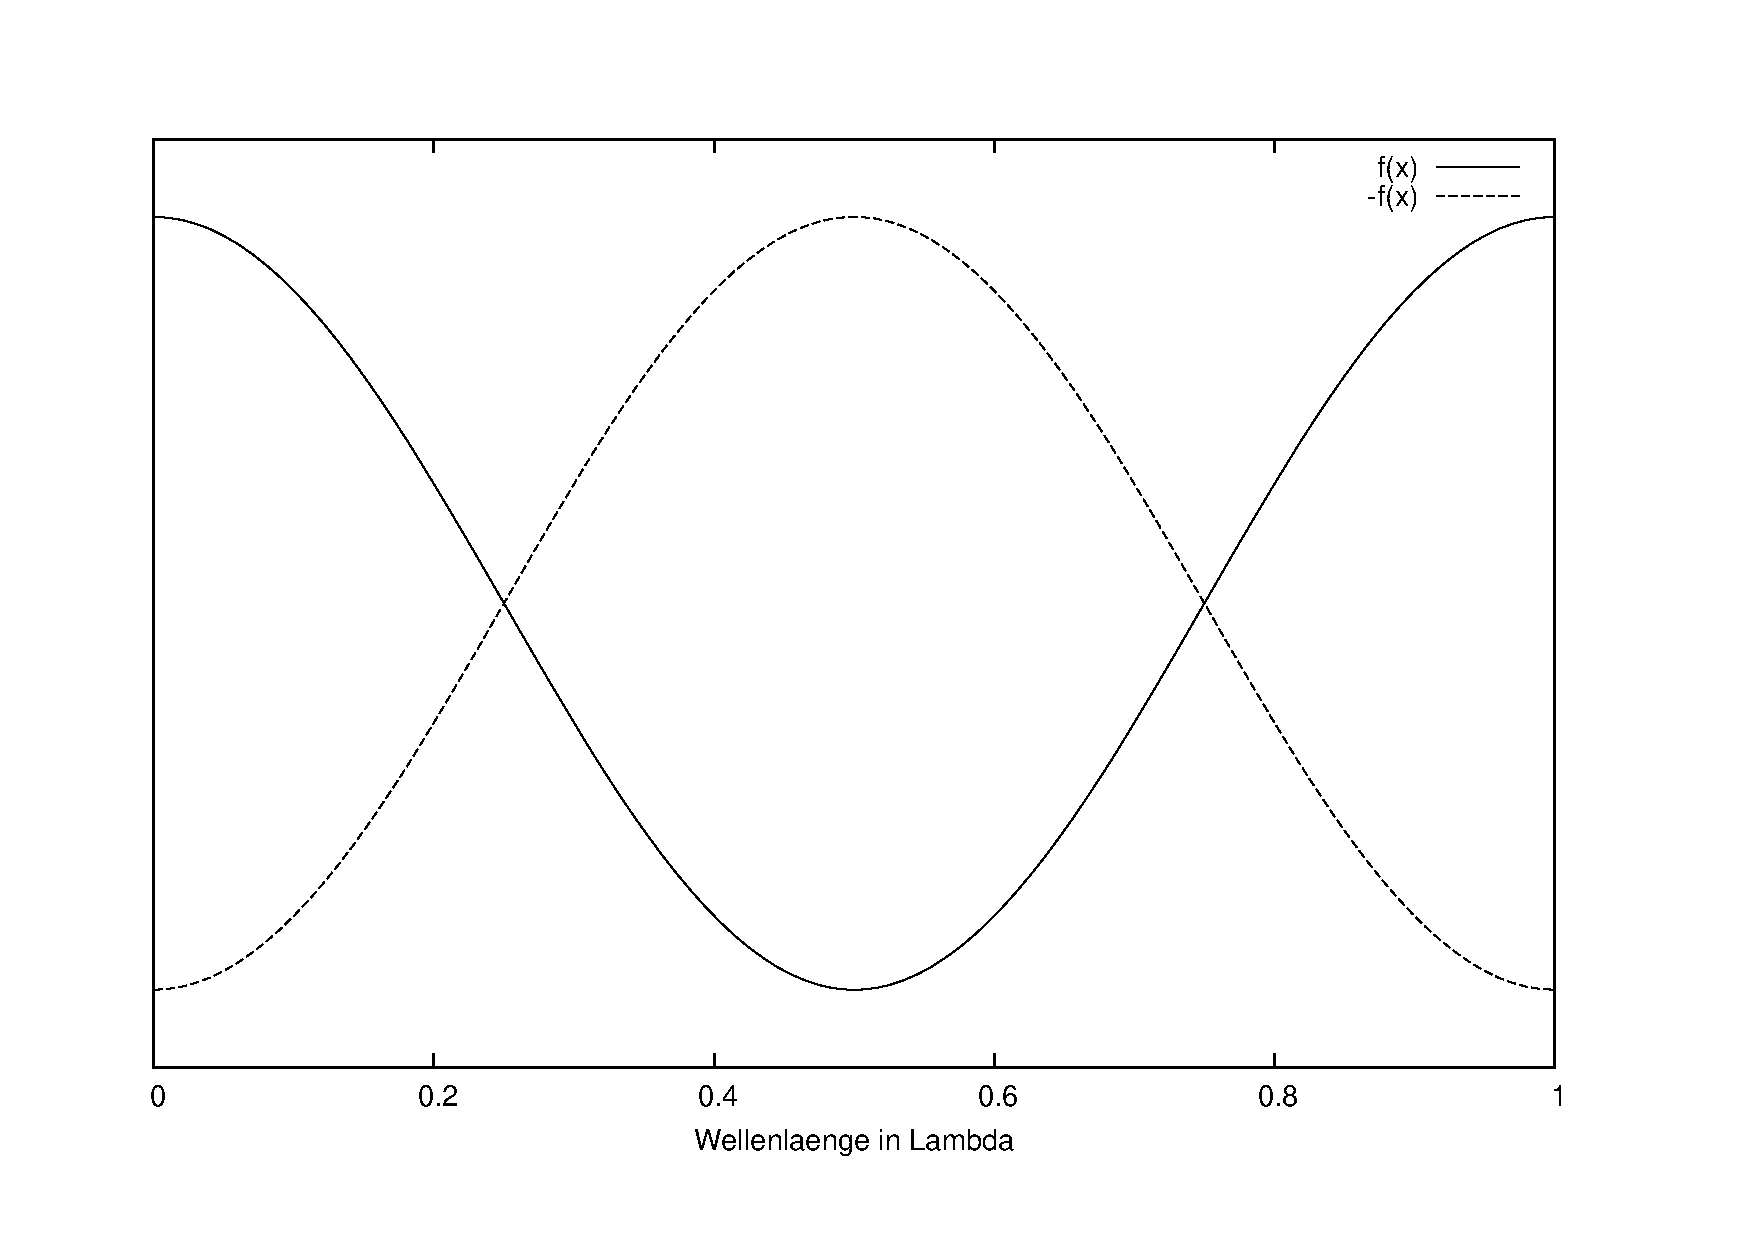
\includegraphics[width=0.4\textwidth]{mat/Q10}}
 \subfigure[Q-x-Diagramm, \(L = \frac{\lambda}{2}\), \(t = \frac{T}{4}\)]{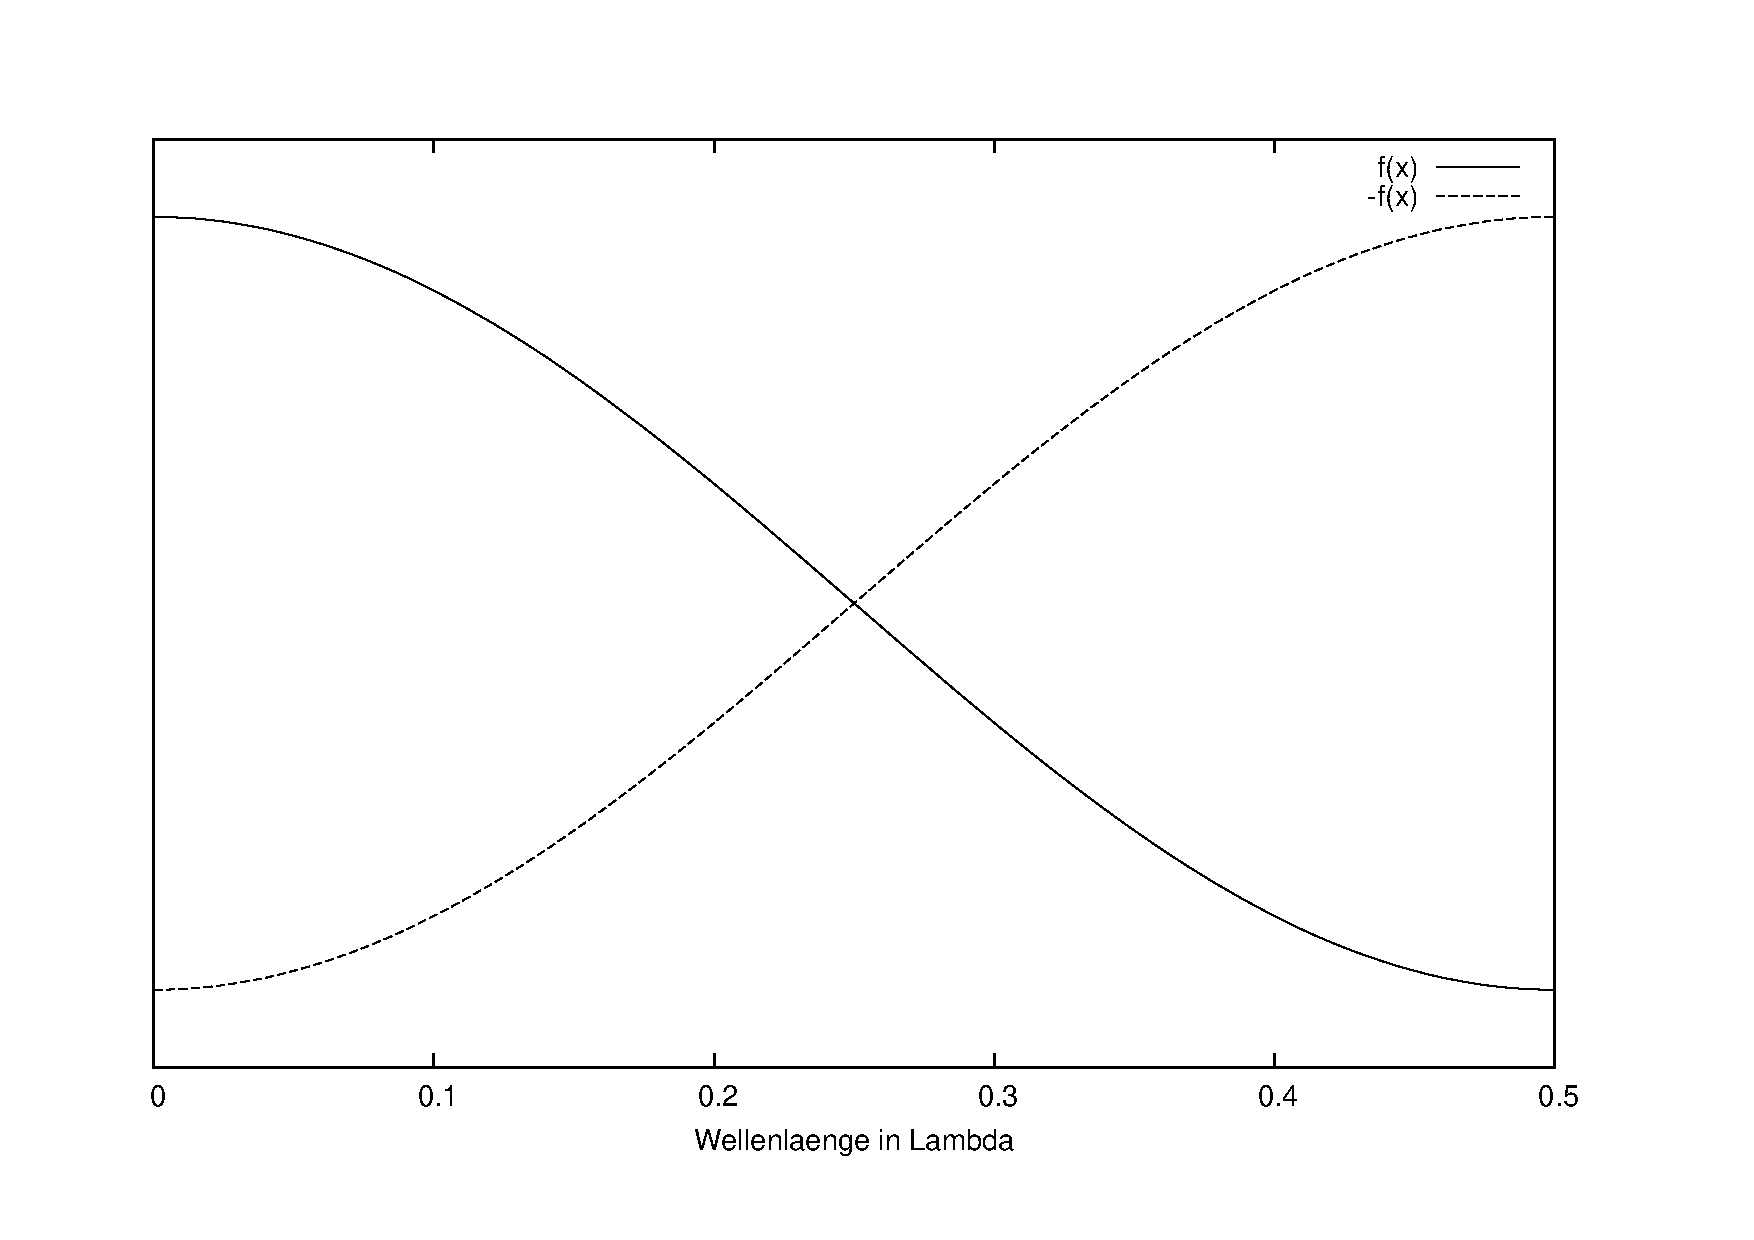
\includegraphics[width=0.4\textwidth]{mat/Q05}}
 	\caption{Stehende Wellen auf einem Empfangsdipol zu verschiedenen Zeiten; entweder Strom oder Ladung betrachtet}
 	\label{img_Ix-Qx}
\end{figure}






		\section{Definition Elektromagnetische Welle}

\index{Elektromagnetische Welle!Definition}Eine elektromagnetische Welle besteht aus einem B-Feld und einem E-Feld die sich durch ihre andauernden Änderungen stets gegenseitig 'erschaffen'. Dabei stehen B-Feld und E-Feld senkrecht aufeinander und gleichzeitig senkrecht zur Ausbreitungsrichtung, es handelt sich um eine \emph{Querwelle}.\footnote{Die von einem Dipol abgestrahlte elektromagnetische Welle ist \emph{linear polarisiert}. D.h., dass die Schwingungen senkrecht zur Ausbreitungsrichtung nur in \emph{einer} Richtung liegt. Außerdem strahlt der Dipol \emph{nicht} in Richtung seiner Achse.}
%Die Längen Vektoren der Felder schwingen dabei nach einer Sinus-Funktion.

Im Nahfeld eines \textsc{Hertz}'schen Dipols wird die Welle noch durch Ladungen und Ströme (mit)bestimmt, ab einer gewissen Entfernung - im \emph{Fernfeld} - jedoch erzeugen sich die Felder durch ihre zeitliche Änderung gegenseitig. Wäre dies nicht der Fall, so müsste die Intensität reziprok kubisch zur Entfernung abfallen\footnote{\(I \sim \frac{1}{r^3}\)} - das tut sie aber nicht. Die Schwingung im Dipol muss aber auch schnell genug sein, damit sich die Felder richtig abschnüren können, also in sich geschlossene Feldlinien bilden, die nicht mehr mit dem Dipol zusammenhängen.



		\section{Ausbreitungsgeschwindigkeit}
		\label{ss_Ausbreitungsgeschwindigkeit}

\index{Ausbreitungsgeschwindigkeit}Auch wenn elektromagnetische Wellen kein Medium brauchen, um sich fortzupflanzen, ist die \emph{Geschwindigkeit}, mit der sie sich fortbewegen vom umgebenden Medium abhängig. Die Frequenz einer Welle bleibt beim Übergang in ein anderes Medium unverändert. Durch die veränderte Ausbreitungsgeschwindigkeit und Formel \ref{eq_cLf} (S. \pageref{eq_cLf}) dagegen passt sich die Wellenlänge der Welle dem Medium an. Es gilt dabei für die Ausbreitungsgeschwindigkeit
\begin{equation}
 	c = \frac{1}{\sqrt{\mu_0 \cdot \mu_r \cdot \varepsilon_0 \cdot \varepsilon_r}}
\end{equation}





		\section{Reflexion und stehende Welle}

\index{Reflexion}Eine EM Welle wird an einer leitenden Wand reflektiert. Dabei baut sich in der Wand ein Gegen-E-Feld auf\footnote{\textsc{Lenz}'sche Regel: Das B-Feld der EM Welle induziert eine entgegengerichtete Spannung in der Wand.}. An dieser Stelle ist somit die Summe des E-Feldes \(\vec{0}\), es liegt also ein \emph{E-Feld-Knoten} vor. Durch die Ladungsverschiebung in der Wand ergibt sich wieder ein B-Feld und somit liegt an der Wand ein \emph{B-Feld-Bauch}.


Durch die Reflexion an der Metallwand ergibt sich logischerweise eine \emph{stehende Welle}, zumindest in direkter Nähe zur Reflexionsfläche. Bei ihr sind B-Feld und E-Feld um \(\Delta \varphi = \frac{\pi}{2}\) \emph{phasenverschoben}.




		\section{\textsc{Maxwell}gleichungen}

\index{Maxwell-Gleichungen}Für uns sind folgende Aussagen der \textsc{Maxwell}'schen Wellengleichungen wichtig:
\begin{itemize}
 \item Bewegt sich ein B-Feld mit der Geschwindigkeit \(v\), so erzeugt es ein E-Feld der Stärke \(E = B \cdot v\). Dieses E-Feld ist \emph{Ursache} der \textsc{Lorentz}-Kraft.
 
 \item Ein sich änderndes B-Feld erzeugt ein elektrisches Wirbelfeld
 
 \item Ein bewegtes E-Feld erzeugt ein B-Feld
 
 \item Ein sich änderndes E-Feld erzeugt ein magnetisches Wirbelfeld
\end{itemize}

Man kann sich die Richtungen der Felder jeweils (logisch) herleiten.\index{Rechte-Hand-Regel} Dazu kann man die rechte Hand verwenden und mit dem Daumen den Feldlinien eines E-Felds folgen, denn so man erhält aus der Richtung der Finger die Richtung des B-Feldes. Um das entstehende E-Feld zu bestimmen, verwendet man das \textsc{Lentz}'sche Gesetz: Wenn aus einem E-Feld ein B-Feld entsteht, so wird dieses stets in die Richtung zeigen, dass das aus \emph{ihm} entstehende E-Feld dem ersten - ursächlichen - E-Feld entgegensteht. D.h. Es muss ein B-Feld entstehen, dem man mit dem Daumen der Rechten Hand so folgen kann, dass die Finger der Rechten Hand dem bestehenden E-Feld entgegenzeigen. 
In dem Fall, dass ein B-Feld sich bewegt, kann man sich der Linken-Hand-Regel bedienen: Das E-Feld muss so entstehen, dass Elektronen in ihm der \textsc{Lorentz}-Kraft folgen würden.





